\documentclass[12pt,a4paper]{report}

% ---------- PACKAGES ----------
\usepackage{url}
\usepackage[utf8]{inputenc}
\usepackage[T1]{fontenc}
\usepackage{lmodern}
\usepackage{setspace}
\usepackage{geometry}        % For margins
\usepackage{hyperref}
\usepackage[most]{tcolorbox} % For your black/white intro boxes
\usepackage{amsmath} % For the arrows
\usepackage{tikz}  % For the figure 1
\usetikzlibrary{arrows.meta, positioning, shapes.geometric} % For the figure 1

% This goes in your preamble
\usepackage{tabularx} % for tables 5.4
\usepackage[table]{xcolor} % for tables 5.4 & appendix tables
\usepackage{longtable} % for tables 5.4 & appendix tables
\usepackage{multirow} % for tables 4.1
\usepackage{ltablex} % for appendix tables
\keepXColumns % for appendix tables
\setcounter{secnumdepth}{3} % fourth level heading 6.2.2.1
\usepackage{float} % table position control esp chapter 6
\usepackage{placeins}% images position [H]()

 %%%%%%%%%%%%% for appendix tables
\usepackage{longtable}
\usepackage[table]{xcolor}
\usepackage{array}
\usepackage{ragged2e}

%%%%%%%%%%%%%%%%%%%%%%%%%%%%%%%%%% Emails line breaks
\usepackage[hyphens]{url}
\usepackage{breakurl}

%%%%%%%%%%%%%%%%%%%%%%%%%%%%%%%%%Appendix B
\newcommand{\appsubsection}[1]{
\par\medskip
\noindent{\color{blue!60!black}\rule{\textwidth}{0.6pt}}
\par\vspace{0.9em}
\noindent{\large\bfseries #1}
\par\vspace{0.3em}
\noindent{\color{blue!60!black}\rule{\textwidth}{0.6pt}}
\par\medskip
}

\usepackage{microtype} % For the margin
\sloppy % For the margin
\newtcolorbox{chapterintro}{
    colback=lightgray!30,      % Grey background
    colframe=black,     % Black border
    colupper=black,     % White text
    sharp corners,      % No rounded edges
    boxrule=0pt,        % No border thickness
    fontupper=\itshape, % Italicized text
    halign=center,      % <--- THIS CENTERS THE TEXT
    top=4mm,            % Padding at the top
    bottom=4mm,         % Padding at the bottom
    left=1cm,           % Extra margin on the left inside the box
    right=1cm           % Extra margin on the right inside the box
}
\usepackage{enumitem}


\geometry{margin=1in}

% ---------- Change tracking ----------
\usepackage[draft]{changes}

\definechangesauthor[name={Grace}, color=blue]{gz}
\definechangesauthor[name={Supervisor}, color=red]{sup}

%\added[id=gz]{new paragraph}
%\deleted[id=sup]{old wording}
%\usepackage[final]{changes}
%\replaced{new text}{old text}


% ---------- Page colouring for now ----------
% 1. Load the packages needed for color management
\usepackage{xcolor}
\usepackage{pagecolor}

% 2. Define a comfortable, soft light orange color (using a Hex code)
\definecolor{lightorange}{HTML}{FFEEDD} 
\definecolor{darktext}{HTML}{2D3748}

% 3. Apply the background color globally
\pagecolor{lightorange}

% ---------- DOCUMENT ----------
\begin{document}

\pagenumbering{arabic}

\tableofcontents

\listoffigures
\addcontentsline{toc}{chapter}{List of Figures}

\listoftables
\addcontentsline{toc}{chapter}{List of Tables}

\chapter{Introduction}

\begin{chapterintro}
This chapter introduces unemployment and the methodology used to approach this research.
\end{chapterintro}

Unemployment is a worldwide crisis affecting hundreds and thousands, with the global unemployment rate at 5.7\% over 2015--2016 and at an alarming 26.7\% in South Africa in 2016. The United Nations thus rightly listed “Decent Work and Economic Growth” as goal number eight of the Sustainable Development Goals (SDGs) with the goal to achieve full and productive employment for both men and women through job diversification and technological upgrade and innovation. Unemployment is thus categorised as an Information Communication Technology for Development (ICT4D) problem; characterized by issues of low-income, illiteracy, marginalisation and other forms of underdevelopment. As expected, unemployment results in several social ills such as increased crime, ill-health and educational inequalities thus widening the gap between the rich and the poor. In addressing unemployment, several applications have been created to tackle the issue, these can be classified as ICT4D interventions. Among these are Ummeli, a website for finding jobs for the unemployed in South Africa and Babajob, a website where job seekers are connected to employers in India.

Job readiness (JR defined in Section 2.2) programs and non-governmental organisations (NGOs) in Cape Town address the unemployment problem through upskilling but lack ICT4D interventions. JR graduates still face issues such as poor search skills, lack of mobile devices and data to access job opportunities. Thus, Co-design features as an approach to offers an opportunity to work with these NGOs to identify where ICT4D expertise might play a role and offers a platform to work directly with the affected stakeholders to design and evaluate solutions. In this research, we used Co-design to understand unemployment and explore ways in which ICTs can be used to ease job searching for job seekers. By using Co-design, we are able to make use of a combination of different tools and methods to engage our users, flexibly move between cycle phases and gain rich user-oriented suggestions and solutions. Thus, we interchanged between the use of participant observation, surveys, one-on-one discussions and workshops as was needed for the different enquiry and design stages.

The first cycle of our research was focused on discovering and understanding our users’ capabilities and their usage of communication and networking technologies, which are used in job searching and other everyday tasks. In Cycle 2, we worked together with our users to (1) design an enabling artefact to assist with job finding, and then (2) develop a working version of the artefact. Finally, in Cycle 3, we deployed the improved version of the artefact for a period of two weeks and assessed its feasibility and potential impact.

Through our research, we worked with job seekers, who we recruited at two JR training sites as well as their trainers to grasp the issues around unemployment in Cape Town, South Africa. From our findings, we discuss the combination of technologies and approaches to tackle the problem; mobile and web-based methods, door-to-door and electronic searches, SMS and email communications for job searching for the low-skilled. We discovered our users’ preferences as well as the barriers to using the preferred mode of communication. Finally, we deployed an application which combined some of our users’ different means of communicating and job finding, as well as existing best practices of job search sites.

Our two NGO partner organisations: Afrika Tikkun and The Zanokhanyo Network are both organisations focused on attracting unemployed individuals who are seeking to become more employable, by providing them with JR classes, which are classes which prepare them for the world of works. Our research involved two different organisations to improve the rigour of our outcomes. Our participants were: job-seeking students as beneficiaries, their trainers as intermediaries and the researcher as an observer, interviewer, data analyst and software developer. All three stakeholders worked together as Co-designers in the design process of the eventual artefact.

We discovered what worked and what did not work for the low-skilled job seekers and went on to develop and deploy an application to access its practical feasibility. Through the research, several trade-offs affected our findings and thus we list them for guidelines for future work with unemployed individuals and future work in Co-design.

\section{Research Question}

{\setlength{\parindent}{0pt}
\setlength{\parskip}{1em}
\setlist[enumerate]{leftmargin=*, font=\bfseries}

In this research, we sought to understand the ICT setbacks for employment amid the low-skilled. Thus, we ask:

\begin{enumerate}[label=RQ\arabic*:]
    \item \textit{In what ways are the low-skilled using existing ICTs to find jobs?}
\end{enumerate}

Question one allows us to understand how existing ICTs fit into the lives of job seekers so as not to bring in off-the-shelf solutions which are not usable for our users.

\begin{enumerate}[label=RQ\arabic*:, resume]
    \item \textit{What are the barriers to the use of ICTs for job searching for the low-skilled?}
    \item \textit{Which technology or technologies are appropriate for low-skilled job seekers to find jobs?}
\end{enumerate}

Question two and three then help us to identify the gaps in the current technologies and go on to identify new technologies or new combinations of existing technologies to bridge the gap. To bridge the barriers or gaps we interact with low-skilled job seekers to determine what is appropriate for them by discussing their experiences, preferences and abilities through a series of tools and techniques.

Then we ask:

\begin{enumerate}[label=RQ\arabic*:, resume]
    \item \textit{What are the salient design requirements for ICTs used to assist job seekers in job finding?}
\end{enumerate}

Through the various interactions we were able to determine which issues arose more frequently, i.e.\ which were salient, thus, we contributed to understanding job searching among the low-skilled and other marginalised users with similar technology limitations.

Finally, we asked:

\begin{enumerate}[label=RQ\arabic*:, resume]
    \item \textit{What are the trade-offs to be made when performing Co-design with low-skilled, unemployed or marginalised individuals from NGOs?}
\end{enumerate}

Because of the various methods used to interact with our users, we were able to discuss the trade-offs, in other words: which techniques or approaches worked better under which circumstances and to what extent various methods should or should not be applied. Thus, contributing to understanding Co-design and NGO engagement in ICT4D projects.
}
\chapter{Background}

\begin{chapterintro}
This chapter gives information about the organisations the researcher worked with as well as background information about unemployment and job readiness (JR) programs.
\end{chapterintro}

\section{Context: Unemployment in South Africa}

The United Nations Sustainable Development Goals names “Decent Work and Economic Growth” as goal number eight, noting that widening inequalities has led to slow job creation, with over 204 million persons unemployed in 2015. There are many factors that cause unemployment: slow job creation, educational inequalities and social instability. In South Africa in particular -- there are many more unskilled labourers than positions available for them, while positions requiring skilled labour often go unfilled. These potential employees, further, face many barriers to employment. Transport costs are exacerbated by geographic inequalities persisting from forced relocations during apartheid. Reliance on an unreliable transport system deepens their difficulties; transport to and from work takes a long time, and train delays make them late for work despite early starts. Youth and foreigners especially struggle with language inequalities; from online job postings, many employers require fluency in English and Afrikaans, rather than isiXhosa, which is the medium of teaching in many township-based schools, or the native languages of African refugees seeking employment in South Africa. Finally, foreigners face difficulties getting visas to work, forcing them to take informal employment at wages below living costs, affecting their performance at work and their ability to retain jobs. At the same time, because of word-of-mouth based recommendations, those that can get and keep a job for a year are often those that stay employed for the rest of their lives.

\section{Job Readiness Programs}

Many non-governmental organisations (NGOs) address unemployment through job readiness (JR) programs, which provide soft-skills training to help their participants improve their English, learn how to obtain and keep jobs, and seek additional training in specific trades. These programs include some computer skills training, often necessary for curriculum vitae preparation and for finding available posts online, but also a valuable skill in general, making learners more employable. In this section, we describe the JR programs of our two partner NGOs.

\subsection{The Zanokhanyo Network (TZN)}

The Zanokhanyo Network (TZN) is a non-profit organisation targeting unemployed individuals. TZN assists to provide employee-sought skills and self-confidence boost amongst other benefits to all kinds of job seekers, both foreign nationals and locals. We focused primarily on TZN’s Wynberg site, which serves people of various ages from all over Cape Town, including many French-speaking refugees. Other courses offered in this site include a basic English language course, computer skills training, waiter/waitressing, and barista courses.

The JR course runs over a 12-day period in which the following modules are delivered:

\begin{enumerate}[label=\textbf{\arabic*.}]
    \item Who am I?
    \item Emotional Healing
    \item Why character matters
    \item Introduction to computers
    \item Stumbling blocks on the journey, but God\ldots
    \item Self-management
    \item Searching for employment
    \item Applying for vacancies
    \item Getting your job
    \item At the workplace
    \item Landmines in the workplace
    \item Beyond Job Readiness
\end{enumerate}

After completing the course, the JR graduates are invited to return any time to make free use of the resource centre, which is an internet-connected computer lab. The JR classes were offered for R60 (~\$5) per student. The job readiness classes are few to enable the students to cover the whole syllabus before rushing to find a job, also to reach as many students as can be reached annually, which is in line with South Africa’s vision 2030 of providing one million learning opportunities through community education and training centres \cite{npc2013}. The more students reached by each job-readiness programme, the quicker the goal will be reached.

\subsection{Afrika Tikkun (AT)}

Like TZN, AT is an international organisation that trains individuals to become ready for employment. AT works in partnership with SEDA and ESKOM. AT runs three core programs suited to different age groups:

\begin{enumerate}[label=\textbf{\arabic*.}]
\item Early Childhood Development program
\item Child and Youth Development program
\item Career Development program
\end{enumerate}

In this research, we focus on the Career Development Program, which is a two-month JR program, which targets 19--35 year old individuals. The NGO trains individuals by providing them with money skills, people skills and work management skills. AT runs their JR classes at Mfuleni, a township nearly 40km from Cape Town. The readiness classes are offered free to the students.

\section{Participatory Design for Development}

Participatory Design is a design approach that attempts to obtain bi-directional knowledge transfer between users and designers (Information Technology experts), for users to have a say and allow the designer to make the possible approaches to solving problems known to the users. Although PD was targeted at office work \cite{simonsen2013}, it has shifted to use in research. PD allows users to be more engaged, “having a say” \cite{simonsen2013} as opposed to being “spoken for” by the researcher \cite{frascara2002} in a user-centred design approach. In PD the user is recognized as an expert \cite{bjorgvinsson2010}.

PD involves in-depth knowledge often from few individuals, as such PD has sometimes been criticized as being small scaled and short-lived \cite{simonsen2013}, mapping only to a small or local context and dying once the project is completed. We acknowledge this criticism as a critical ethical issue for both PD and Co-design; however, we reduce the chance of running into this issue by working with NGOs as partners capable of disseminating information about and mediating the use of artefacts generated during research over different intakes of students.

\section{Co-design for Development}

Co-design is a process of collective creativity throughout the design process \cite{sanders2008} among different kinds of experts \cite{steen2011}.

Like Co-design, Participatory Design (PD) is a design approach that attempts to obtain bi-directional knowledge transfer between users and designers. However, Co-design has a significant difference in that all participants are considered equals in the design process, irrespective of their role \cite{zimmerman2011}. Allowing equity for all participants ensures that the non-IT-experts, in this case job seekers, can have a strong voice in the design process.

The participants in Co-design can be academics, researchers, designers or other professionals; however, all are experiential experts, that is, experts of their own experiences \cite{steen2011} and of their preferences \cite{preece2002}, which are useful for coming up with designs and choosing among multiple designs.

In terms of living labs, there are two “research types”: observation research, where a user is considered as a subject, and participative research, where a user actively contributes in co-creating value. Our methodology, Participatory Design, and our design approach, Co-design, both fall under participative research \cite{pallot2011}.

We consider job seekers as experts in understanding the challenges in job searching and as such should be deeply involved in the research and not just be informants. Engaging users early in the design process allows users to be more likely to identify issues that can be met by technology usage and increases their likelihood to adopt a design solution into their practices \cite{david2013}.

Co-design is very critical to research that is aimed at development because although some values are known with little input directly from participants, not all values are explicit and common to individuals. Co-design provides a setup where users can be challenged by other users or through the performance of certain tasks to express themselves \cite{halloran2017}. Co-design enables several benefits: it fosters joint creativity \cite{steen2011}, induces ownership and sustainability \cite{david2013}, and promotes the generation of inspired ideas through probes \cite{sanders2014}.

In our Co-design cycles, we make use of various tools and techniques such as workshops, interviews, walkthroughs and participant observation. The Co-design methodology promotes new ways of engagement and as such should be flexible to change \cite{sanders2008}. Thus, we make use of the Tell $\leftrightarrow$ Make $\leftrightarrow$ Enact Co-design cycle which is flexible to design phase changes.

We aimed to achieve beneficiary empowerment \cite{ssozi2016}, stakeholder equity \cite{zimmerman2011}, cost optimisation \cite{steen2011} and project sustainability \cite{david2013}, which are all possible when using the Co-design methodology.
\chapter{Literature Review: ICT4D}
\begin{chapterintro}
This chapter gives discusses the related works in unemployment and Development.
\end{chapterintro}

\section{Development and Co-design}

Development is “the process of improving the quality of all human lives and capabilities by raising people’s levels of living, self-esteem, and freedom” \cite{todaro2015}. However, to improve the living standard/ “people’s levels of living” \cite{todaro2015} there is a need for money and other resources. To earn money or acquire resources, one needs to be employed or own a business. Various forms of technology are being increasingly seen as enablers of development \cite{npc2012}. However, development often advances with great imbalance, often termed -the digital divide \cite{feldmann2003, sambasivan2010, nicola2011}. In South Africa, the digital divide has been very great, causing a major disparity between the rich and the poor. As with the digital divide, there is also a great disparity in the unemployment rate in South Africa across different groupings. 

The South African unemployment level stands at 25.2\% in 2014 by the strict definition of unemployment. However, there is a great disparity in the unemployment levels when analysed along the groupings of race, age groups and skill levels. Zeroing into the unemployment level among the youth in South Africa (aged 15--24), the unemployment rate is higher, at 36.1\% and further zeroing into the black African youth in South Africa, the rate is even higher, at 39.4\% by 2014 \cite{statssa2015}. South Africa has the goal of slashing down unemployment to merely 6\% by 2030 \cite{npc2012}. These statistics indicate the nation’s need to pay greater attention to the unemployment issues among the youth and in the black communities in order to reach the 6\% mark. 

In South Africa, the financial services, information technology and business services have grown employment, however, mainly for the skilled \cite{npc2012}, thus a need for great efforts in the inclusion of the marginalised individuals. Technologies are generally considered unimportant in underdeveloped communities unless the technologies will contribute to the economic emancipation of the underdeveloped \cite{lorini2014}. 

South Africa is faced by a shortage of skilled labour, which raises the income of the skilled and thus increasing the wage inequality in the country \cite{npc2012}. The newly emergent field of Information Communication Technologies for Development (ICTD/ICT4D) has had several researchers investigation how to alleviate the inequalities: The Farming improvement project to provide agricultural information to farmers \cite{gandhi2007}, money transfer \cite{dyson2007}, job finding information \cite{qiang2012, chepken2012tele}, business starter software for under-developed start-ups \cite{brittan2011}, water service delivery \cite{ssozi2016} and many other infrastructural improvement and information access systems. The recent money transfer system MPESA which makes use of mobile technology to send money has been used by 14 million Kenyans, with transactions to the worth of 7 billion. These systems all aim to diminish the imbalances between rural and urban co-existent communities through the use of information and communication technologies. ICT4D/ICTD is a young discipline that focuses on ICT initiatives that contribute to social or economic development \cite{chepken2012trends}, usually targeted at poor regions of Africa, Asia and Latin America \cite{chepken2012trends}. ICT4D projects have been critiqued for being a cover-up for political agendas from those in power, thus ICTD projects should transparently state action plans, beneficiaries and benefactors \cite{elkhatib2015}. However, South African has identified the great potential in ICTs as listed in the national vision 2030 \cite{npc2012}. Although ICT4D has dated back to the 1990s, we understand it as an academic discipline as well as a field of practice in which Information and communication technologies are utilised to aim at development \cite{chepken2012trends}. In many past studies, ICT4D has been used to aid projects around health, education, agriculture and social communication \cite{david2013, chepken2012trends}. 

The Co-design approach to developing technology helps in improving people’s wellbeing, reducing creation costs (by engaging their very own ideas), and improving the adoption of technology \cite{steen2011}. Co-design can be perceived as a new term for Participatory Design or an improved version of participatory Design, its key principle is the involvement of all stakeholders in the design process to ensure that the end-products meet the users’ needs, are highly adapted and are sustainable \cite{david2013}. Co-design has become integrated with developmental initiatives because of two intersecting ideas: firstly in design, a move toward user involvement for product improvements and secondly, in development, a move towards social embeddedness of projects and the importance of locals in technology appropriation \cite{david2013}. The discussions around Co-design has five main aspects of consideration: stakeholders, context, ownership, social learning, and sustainability \cite{david2013}. In other words, Co-design is about selecting a representative set of stakeholders, performing design within end-users’ contexts, knowing artefact is owned/adopted, obtaining mutual learning and having ICTs that run on a long-term basis. 

\section{Causes of Unemployment}

Gitau attributes the unemployment problem to a lack of skills among the low-income \cite{gitau2012}. In addition, minimum wage and work conditions restrictions from bargaining councils and wage boards, which are applied uniformly irrespective of company size incur relatively higher labour costs on small businesses, \cite{kingdon2001}, which means that small business would not be motivated to employ many workers. This is true for the small subset of individuals who manage to enter the labour force, however, it is suspected that barriers such as disempowerment and restrictions of past apartheid period, lack of infrastructure, land and capital would bar unemployed persons from employment. Poverty discourages job-search activities, \cite{orkin1998} because searching for jobs incurs transport costs, CV creation costs and sometimes data costs. 

Meissner and Blake attribute unemployment to weaknesses in career guidance support that young people receive from the school and family \cite{meissner2011}. In their work, Meissner and Blake made use of personas to show that low-income community youth face challenges of family pressure to find jobs as soon as possible, low or no guidance on how to propel their careers as well as a need to manage the highly-constrained resource, time. The young individuals had to juggle between school and watching over younger ones, or between working and watching over younger ones. They proposed to address this problem by offering career guidance which involved using a computer and website, but also admitted that these individuals were time-constrained and lacked advisors who would give them advice when using the websites.  

Furthermore, research has shown that users with low education levels prefer to receive job notifications through their phones, via SMS or call as opposed to via emails \cite{white2012}. This indicates that they prefer simple mobile technology over computer-based or other advanced technologies. Individuals without college-level education tend to perform worse on computer-based solutions than those of college education level \cite{algarin2009}. However, email addresses are often requested or required on job searching apps and websites like Gumtree (gumtree.co.za), Indeed (indeed.co.za), and Freelancer (freelancer.co.za), thus, they are not directly suited to low-skilled persons. Thus, the proposed intervention in this dissertation should allow unemployed job seekers who are often low-skilled to use their accessible or preferred technology means. 

Moreover, Donner and Gitau identify an important category of technology users: mobile-only users \cite{donner2009}. Mobile-only users do not have the luxury of doing tasks with the most optimised devices (e.g. PCs for typing and video calls and mobile phones for making voice calls) because they have mobiles as their only means of communicating and task completion. These individuals could be better developed for, in a fashion that enables them to understand technology without the need to understand desktop computers. 

Meissner uncovered that users would like the best-paying jobs rather than the most fulfilling job, the findings also included that users do not get information about tertiary education and jobs frequently enough, and job availability information was sometimes outdated \cite{meissner2011}, highlighting the demand for relevant information and to access the information quickly \cite{bhavnani2008}. 

Since job seekers face so many challenges including the discussed: lack of skills, transport cost, CV creation cost, data cost, minimum wage and work conditions restrictions from bargaining councils and wage boards, and restrictions of past apartheid period, lack of infrastructure, land and capital, poverty and poor career guidance it is evident that that unemployment is a multidimensional issue which requires various agencies to tackle it. 

\section{ICT Interventions for Unemployment}

Several projects have attempted to use ICTs to tackle unemployment and poverty problems. Ummeli \cite{gitau2012} is a text-based mobile unemployment solution that was targeted at semi-literate individuals. We discuss this application because it was developed specifically for use in South Africa. Ummeli provides functionalities for its users to browse for jobs, post jobs and recommend jobs, create CVs and communicate with other job seekers. It was tested in the South African township of Khayelitsha \cite{gitau2012}. However, the application was registered for Vodacom cellular network users only. This meant that other unemployed candidates registered on other cellular networks such as MTN and Cell C would be left out. Babajob (babajob.com) is a job searching network that connects job seekers to employers, particularly connecting poor job seekers with few skills to elite employers. Babajob utilises cell phone numbers to register job seekers as an alternative to email addresses; and involves people, who may guide the use of technology by non-experts. Babajob’s interface is simple with very few steps required from a job applicant as opposed to Indeed and CareerJet job search platforms. Babajob also allows users to apply directly through the site, as well as subscribe to get SMS \cite{babajob2016}, however, the facilities are local to India.  

Like Babajob, Giraffe (giraffe.co.za), which is a job searching platform based in South Africa allows mobile numbers to be used to create an account. However, Giraffe has the shortcoming of requesting for South African identity numbers which then bars non-South Africans from accessing the job opportunities available through the website. 

Greataupair (greataupair.com/search/hire.cfm/careType/nanny) is another good website for job finding, which filters job seekers by age and salary, the website posts jobs and job seekers, however, it is designed specifically for housekeeping jobs. Greataupair requires an email to register an account. Like Babajob, the Kazi560 application in Kenya is an example of an application that successfully improves the lives of job seekers, job seekers can subscribe to SMS messages for a small fee per SMS \cite{qiang2012}.  

The Indian government announced the National Skills Development Policy, which aims at creating 500 million skilled employees by 2022, amongst its other goals. Thus, in Karnataka, India, the labour department implemented a national network of employment centres across the country where ‘candidates’/potential job seekers undergo an assessment of their background and skill-level and based on the outcome of the assessment, the centre identifies appropriate job vacancies or suitable training for the candidate. The centres are also reachable by calling in to speak to an agent or utilizing a government managed internet portal associated with the centres. Although the approach is sound, the state is unable to maintain the level of assistance required to reach their employability to the goal of creating 500 million skilled employees by 2022 and thus there is huge potential for technology solutions to improve the accessibility of employment services of the centres \cite{white2012}. Similarly the South African government has implemented the National Youth Development Agency (NYDA) to assist South Africans under 35 years with skills training, business start-up guidance and venture capital \cite{nyda2015}, yet like with Indian employment centres, the candidates reached through NYDA are limited, and huge numbers remain unemployed in the communities \cite{statssa2015}. 

Yet with the presence of several mobile interventions around unemployment, mobile Applications for Agricultural and Rural Development (m-ARDs) face challenges of finding funds to run. Several models of m-ARDs are therefore based on obtaining funding through SMS revenues which are low and often must depend on the external support of policymakers and government aid. Particularly in developing regions, m-ARDs face the challenges such as lack of local content, poor quality of available interfaces, influential powers due to monetary support, and because asymmetric access to information is often scarce in these regions \cite{qiang2012}. For example, employers having persistent access to internet and web platforms to post vacancies whereas job seekers are not always well empowered to post their profiles in order to market their skills. Voice-based systems can be utilised when working with the textually illiterate as has been successfully used in a rural setting in India to help individuals find employment \cite{white2012}. 

Some have proposed microtasks as an employment \cite{mtsweni2014, zyskowski2015}. Microtasks are small tasks often taken out of larger tasks and offer compensation to individuals from around the world \cite{mtsweni2014}. Examples of microwork include image location, item classification, translation and survey filling. Microtasks are offered on different microtask platforms accessible through smartphones, and other internet-connected devices. The following are examples of microtask platforms: Amazon’s Mechanical Turk (Mturk), InnoCentive \cite{innocentive2017}, Ajira, Jana and Samasource. However, research in a rural township in South Africa has shown that the community members mainly did not have computers and do not consider smartphones as a potential resource for income generation, as such ruling out their access to microtasks through smartphones \cite{lorini2014}. Microtask platforms offer job seekers non-traditional avenues to seek employment often with payment known upfront. Despite the great potential of microtasks to assist in unemployment, its accessibility is highly hampered because it is often presented in a digital form to be accessed with computers and internet connectivity which many low-skilled job seekers do not have \cite{gupta2012}. Mturk \cite{mturk2018} and TaskRabbit \cite{taskrabbit2013} are based in developed regions and restrict international workers from their use. Samasource obtains its tasks from the developed regions and makes them available in developing countries such as Kenya, South Africa and Uganda. Jana which started off as a small-scale microtask platform in Kenya and Rwanda \cite{eagle2009} has since been scaled-up for use in large organisations around the world, such as CNN, Unilever and United Nations. Jana is well suited to the developing regions in that it makes use of SMS which is cheap and USSD which does not incur any costs.

\section{Is Mobile for Development?}

In recent years, mobiles have become the most easily accessible and ubiquitous device for communication in constrained settings \cite{bhavnani2008, gsma2014}, and as such technologies should be built around the use of mobile devices for access to information and economic markets. Society has experienced a high recent rise in the use of mobile phones, in 2002 mobile subscriptions overtook fixed-lines \cite{feldmann2003}, mobile devices have many advantages which make them desirable. Mobiles are wireless, portable, have the affordance for intimate and personal control and are capable of supporting discrete digital tasks which can be interlaced \cite{donner2015}. Mobile devices are also useful for mobile money transfer \cite{donner2015}, however, the low-end devices/ non-programmable mobile phones do not allow for advanced USSD money transfer systems such as M-PESA \cite{chepken2012tele}. 

A study that involved job-seekers in Cape Town, Johannesburg, Nairobi and Windhoek indicated that although the job-seekers were able to use messaging and call services, they often did not have enough airtime on their devices, with an average of ZAR one in Cape town \cite{chepken2012tele}. Smart mobile devices are also useful for accessing the internet \cite{donner2013}, however, their usage does not override the need for computer-based internet access or Public Internet Access venues (PAVs) \cite{donner2013}. Wireless solutions have some advantages over their wired counterparts, they are faster, speedy to set up and also cost less; however, this is an underestimate when the cost for towers and solar power systems are included \cite{feldmann2003}. 

Intermittent (on and off) mobile data connection can be caused by device battery life, airtime balance, movement between places, changes in signal and congestion \cite{donner2015}. Finding a solution around all the possible causes of intermittent access would simply be infeasible but being knowledgeable about them can motivate the design of solutions that are mostly offline, battery conserving, and cost-effective, moreover, utilising airtime-less peer-to-peer communications (such as Bluetooth), and generally avoiding data intensive interactions.

\section{Including the Masses}

ICTs have great potential in disseminating information timelier and cost-effectively \cite{elijah2006}, however, acknowledging and designing with the knowledge that, communications are often braided \cite{densmore2013} over different channels is essential. The possibilities of channels in braided communication include SMS, Emailing, voice calls, video calls and social media, it is this important to develop solutions that cross platforms or better yet, solutions that are platform independent \cite{molapo2015} because developing an ICT that is suited for only one channel of communication or only a specific device can result in exclusion of people who frequent other channels and devices to communicate. 

The value that a user gains by being provided with new technologies depends on how well the technology fits into the user’s lifestyle (communicative ecology), in some instances new technologies may improve the lifestyle of its users when there is a small learning curve. This reinforces the need for simplicity as identified as a major HCI enabler as is reflective of Schneiderman’s 5th, 6th and 8th principle \cite{shneiderman2004}.

\section{Human Empowerment \& IT Sustainability}

Human empowerment is crucial for the sustainability of an intervention. Vancouver found that users will contribute to a system if they perceive intrinsic motivation such as having fun or helping people they feel affiliated with \cite{zimmerman2011}. In the Ummeli research, Gitau identified the most pressing needs of the participants was to locate and apply for jobs online, however, their going online was not exclusively for job finding but also for entertainment or entertainment-fostering purposes such as finding music, crafting profiles, sending birthday invitations, and befriending people \cite{gitau2012}. Co-design induces a sense of ownership as well as sustainability in a community \cite{david2013}, which is a result of the high engagement in every possible phase of participatory research. A sense of ownership of technology can be an empowerment realisation and sustainability reinforcement. However, in some cases, a technology system may require maintenance, in part by an IT expert or intermediary, and thus each developer should do a good job so that any developer to be able to maintain or build onto, in the case that the system is deemed valuable enough to be continually maintained. Heimerl and others found that it is important to empower a community to solve its own problem with existing knowledge and infrastructure \cite{heimerl2015}. 

Information dissemination is a crucial aspect of empowerment \cite{chepken2012tele}, for example, an artefact that informs people of vacancies and teaches them lessons useful for the work they would like to be employable for can be useful. Surfing the Internet is one way in which people can access information almost anytime, however, the ability to surf the internet is inhibited by the lack of know-how \cite{lorini2014}, mobile access (small sized devices and gesture inconveniences) and search engine results and presentation format. In a recent study with individuals who were semi-skilled and preferably looking for skills training, 60\% of the individuals indicated that they did not find satisfactory information, as search engines did not offer relevant information, did not limit the results to information within their geographical location and gave an overwhelming number of results when they were looking for training courses \cite{paihama2016}. Obtaining ten results was overwhelming for the participants, however, when the number of results was reduced to four, the participants were able to complete their tasks. Because of the shortcomings of search engines and search engines users’ inabilities to search efficiently, word of mouth or person to person communication can be more relevant for finding job opportunities and skills training services. 

A system can be sustainable either by self-maintaining or being human maintained. Having a self-maintaining IT system is close to impossible, in a society where information changes in unpredicted ways whereas human maintenance is possible and feasible. Ensuring that users derive value from the maintenance of a system can motivate them to keep maintaining it. \cite{schwartz2013} found that the unintended uses of devices may motivate users to maintain devices, to learn advanced tasks and possibly instil a sense of ownership in users. A sense of ownership can reinforce freedom and lead to empowerment and sustainability. However, when the empowered individuals are not IT specialists a system may need to be maintained by a specialised IT expert, and thus the system would not be completely sustained by the users, however, if the users are empowered enough they could deem the system valuable enough to invest in getting an external party to maintain it. 

Sustainability can also be approached by ensuring the design of an artefact is not only with affordances for functionalities but is also afforded to let users know of its affordances \cite{mcgrenere2000} as opposed to, having hidden affordances. Designs should be useful for new users, easy to maintain and documented in a way that they can be built unto.

\chapter{Methodology}

\begin{chapterintro}
This chapter details the research method of enquiry: Participatory Co-design. We discuss the participation and activities in each research cycle.
\end{chapterintro}

\section{Tell-Make-Enact Co-design Cycle}

\begin{figure}[h]
\centering
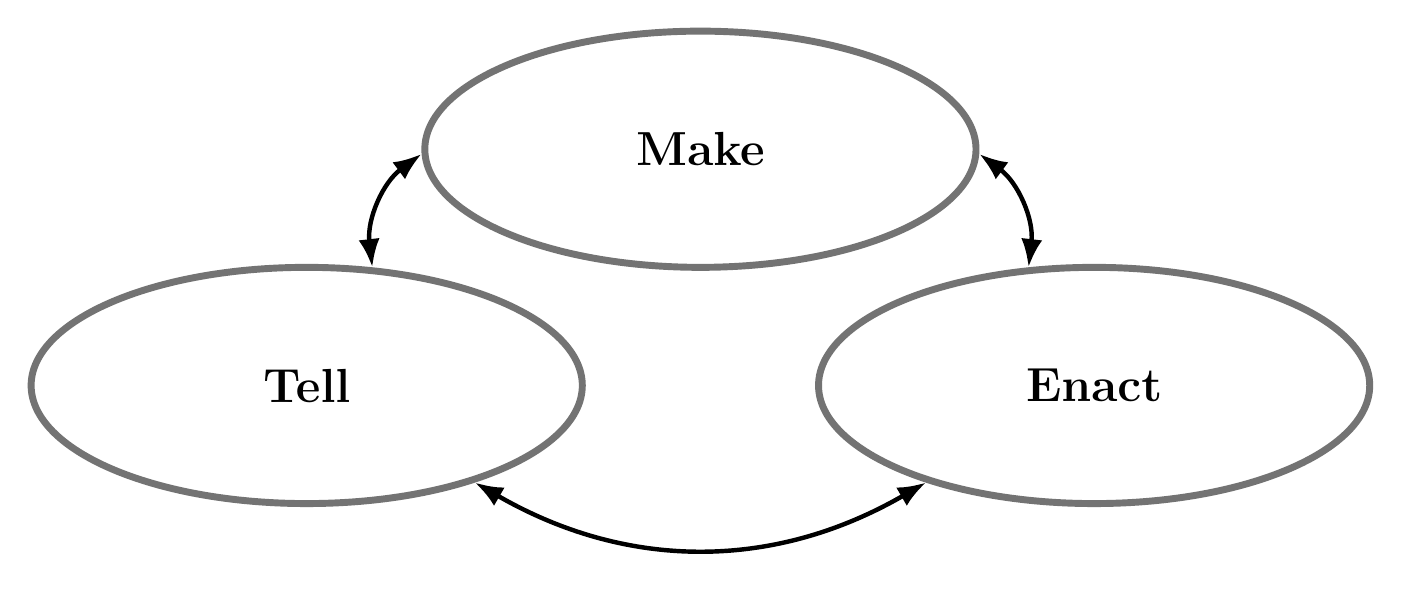
\begin{tikzpicture}[
    oval/.style={
        draw=lightgray!60!black,
        line width=2.5pt,
        ellipse,
        minimum width=7cm,
        minimum height=3cm,
        align=center,
        font=\bfseries\LARGE
    },
    arrow/.style={
        <->,
        >=Latex,
        ultra thick,
        black
    }
]

% Nodes (positioned like your image)
\node[oval] (make) at (0,3) {Make};
\node[oval] (tell) at (-5,0) {Tell};
\node[oval] (enact) at (5,0) {Enact};

% Curved arrows (cycle flow)
\draw[arrow] (tell) to[bend left=30] (make);
\draw[arrow] (make) to[bend left=30] (enact);
\draw[arrow] (enact) to[bend left=30] (tell);

\end{tikzpicture}
\caption{The Tell--Make--Enact Co-design Cycle}
\label{fig:tell-make-enact}
\end{figure}



The research method adopted for this research is Participatory Design (PD) as has been discussed under the sub-heading: “Participatory Design for Development” making use of the tell-make-enact cycle over three iterations. The cycle was coined by Brandt and others \cite{simonsen2013}. Brandt suggests that the traditional participatory action research design cycle of Plan $\rightarrow$ Do $\rightleftarrows$ Observe $\rightarrow$ Reflect is replaced by a Tell--Make--Enact cycle,
that allows prototyping to happen in any stage and acknowledges that design entails movement in both directions around the cycle. Thus, we use the PD methodology with a change in the design cycle to allow for fluid Co-design (designing together on par) with potential users.


\bigskip

\textbf{Tell $\rightarrow$ Make $\rightarrow$ Enact}

\begin{itemize}
    \item \textbf{Tell:} A Co-designer describes an employment-related idea
    \item \textbf{Make:} A prototype of the idea is created
    \item \textbf{Enact:} The prototype is used to generate new ideas and insights
\end{itemize}

\bigskip

Our research focused on trainers and students who were currently taking or had recently graduated from job-readiness programs. In part, this is because we believe that it is important to work with NGOs as gatekeepers in ICT4D projects since they already have programs and relationships with the target population. As a result, they can help provide additional insight. Intermediaries are often trusted and sometimes able to bridge language gaps. In addition, it is difficult to make ICT interventions work in absence of any support infrastructure. We expect that without JR training and access to job-seeking services through the NGO, the participants would not be able to benefit from a specialized application. Working with two organisations allows us to get a broad understanding of the problem, from multiple different perspectives and obtain a collective solution which is potentially very useful for similar contexts around the world.

The research is conducted using participant observation, trainer interviews, student interviews, student workshops and one-on-one walkthrough sessions. We conducted the participant observation as a long-term source of source of unspoken information as well as tacit knowledge. We conducted interviews and one-on-one walkthrough sessions with both student and trainers. During the interviews and walkthrough sessions, we recorded our participants’ dialogues and later transcribed the recordings. We used both NVivo and manual comparison of findings. For the manual comparisons, data were tabulated into columns in Microsoft Excel, where each column represents the same data attribute. I.e. Separate columns for answers to different questions and then comparing the individuals’ responses and suggestions. Some excel sheets of data analysis have been included in the appendices of this dissertation.

\section{Participation}

In this research, we worked with unemployed persons from two NGOs (not-for-profit-organisations). We chose to work with two separate NGOs for our findings to be rich and greatly generalizable. We worked with proactive unemployed persons, those attending the NGO-based JR programs. The job seekers who are mostly low-skilled are sometimes referred to as day-workers as they perform short-term jobs \cite{chepken2012tele, chepken2011}. Limiting our engagement to willing participants from the JR programs. As such, we eliminated those who were not actively looking for jobs, i.e. those who were not present because of family responsibility and those who were not leveraging the opportunities put out by the JR programs.

We expect that the individuals who have attended the JR programs, which included computer learning would be better positioned to leverage a new ICT-based intervention. The exposure to technology, access to computer and internet facilities and the presences of trainers at the NGO sites would assist them in assimilating new technology into their job search. Thus, any technology developed is being used in the context of existing socio-structural resources.

We worked with the NGOs for a period of 18 months. By spending a long period of time with the NGOs, we got a chance to interact with many unemployed students from different intake groups, thus, broadening our understanding of unemployment and technology. In each cycle of our research, we worked with a new set of participants, particularly because the JR programs were shorter than our research cycles, which meant that our participants would have graduated to enter the job searching world before each subsequent cycle. By having different participants in each cycle, we got design suggestions and other feedback from a larger set of participants.

Table ~\ref{tab:research-activities-cycle} gives details on the activities we conducted in each cycle. In the first, we focused on understanding the problem and in subsequent cycles we sought out ways in which one of the problems could be tacked. Outside the formal research activities, the researcher volunteered at the NGO cites to assist participants with computer training, interview preparation and CV creation and proofreading. The interactions allowed the researcher to understand the bottlenecks in the job search process.


\begin{table}[htbp]
\centering
\caption{Research Activities Listed by Cycle}
\label{research_activities_by_cycles}
\renewcommand{\arraystretch}{1.35}
\begin{tabularx}{\textwidth}{
|>{\centering\arraybackslash}p{2.6cm}|
>{\centering\arraybackslash}p{1.2cm}|
>{\centering\arraybackslash}X|
>{\centering\arraybackslash}p{2.6cm}|
>{\centering\arraybackslash}p{2.6cm}|
}
\hline
\rowcolor{gray!30}
\textbf{Cycle} & \textbf{NGO} & \textbf{Activity} & \textbf{Student Participants} & \textbf{Trainer Participants} \\
\hline

\multirow{4}{=}{\centering\textbf{Cycle 1: Needs Assessment}}
& AT & Workshop & 5 & -- \\
\cline{2-5}
& AT & Interviews & 2 & 2 \\
\cline{2-5}
& TZN & Workshop & 33 & -- \\
\cline{2-5}
& TZN & Interviews & 2 & 2 \\
\hline

\multirow{2}{=}{\centering\textbf{Cycle 2: Ideas Focus}}
& AT & Walkthroughs & 6 & 2 \\
\cline{2-5}
& TZN & Walkthroughs & 5 & 1 \\
\hline

\multirow{2}{=}{\centering\textbf{Cycle 3: Deployment}}
& AT & Deployment and Walkthrough & 5 & -- \\
\cline{2-5}
& TZN & Deployment and Walkthrough & 5 (1 incomplete) & -- \\
\hline

\end{tabularx}
\label{tab:research-activities-cycle}
\end{table}




\section{Ethics}

\subsection{Testing a Potential Solution}

Before embarking on any research, the researcher should analyse whether there is a problem or there is an opportunity for improvement. Before the beginning of this project in 2016, the researcher found out that the Unemployment Rate in South Africa was over 25\% in 2016 \cite{statssa2016} and thus, the opportunity to assist in bringing down to the government’s goal of 6\% \cite{statssa2015, npc2013}. 

To understand the problem, we decided to partner with NGOs who focused on training job-seekers who were struggling to get jobs. Through the NGOs, we were able to engage over 50 participants in our project at various stages of the project and to meet over many other job seekers during the sessions when the researcher volunteered to offer the job-seekers, Computer skills (typing, online search, emailing, etc.). 

It was a valid question to ask, should a job-seeker with no source of income be engaged in a project which’s value is in the future? However, we considered it plausible to continue the research as we expected the future value to negate the time taken to take part in the research. However, at the beginning of each session with the job seekers, we let them know that they were free to stop participating at any point and during one of our sessions, one of our workshop participants excused himself to go to his part-time job.

%================================================
\subsection{Hidden Identity and Hidden Aptitude}

Racial segregation, discrimination major unethical issues that occur frequently in society, however, with ICTs individuals are able to avert being segregated because of their skin colour or race as ICTs are capable of hiding identities \cite{chepken2012tele}. 

The usage of hidden identities is positive to avoid discrimination however, ICTs go to the extent of hiding people’s aptitudes as computers and other smart devices perform work that is supposed to be performed by individuals which bring an issue around whether it is fair to hide individuals’ abilities as opposed to expose the potential of the individual (who is in this instance a technology user). 

In job-seeking for example: should an application hide the potential of a job seeker to an employer seeking the best candidate for a task? The issue of hidden aptitude is particularly relevant with blue-collar jobs where an employer has a limited time to test an individual’s abilities as jobs last short periods: hours, weeks and at most, a year where probations do not apply \cite{chepken2012tele}. 

The proposed ‘Employment Service Bill’ of South Africa aims to promote the employment of disabled people \cite{gitau2012}. However, the same ICTs which would hide aptitude would work differently for the disabled and other home-bound people, because it would eliminate tasks that they are no longer able to perform by making use of a different/non-impaired sense \cite{stefano2016} or allow working from a remote area \cite{stefano2016}. However, when individuals work at different geographical locations, it may mean that some will have to work at night or during unsociable hours \cite{stefano2016}.  
%==================================================
\subsection{Compensation}

Compensation or remuneration given to research subjects for participating in research projects is useful as a form of motivation \cite{zimmerman2011, ssozi2017} in addition to the intrinsic motivation to solve the problem at hand. Similarly to other ICT research, we compensated participants with food \cite{winschiers2009} and airtime \cite{gupta2012}.


In some instances, compensation to the research subjects serves both the researcher and the subjects, for example in rural Uganda participants were given phones for use for the research’s goal as well as personal use and the participants felt they gained social status in the community by having phones which were better than other community members’ phones. In India including users in videos was used as both incentive to motivate their participation and as an aid to the adoption of the tool for others \cite{gandhi2007}, thus the form of compensation helped the effectiveness and sustainability of the project.  

Although we did not experience the bidirectional benefit of compensation, in this research we found that the volunteer work that the research did with the job seekers made some of them more willing and more comfortable to participate in our research, such that most of them volunteered to be part of the research. In cycle 2 when participants were not compensated, the \replaced{researcher}{research} struggled to get enough participants.

\section{Cycle 1: Understanding ICT Use and Unemployment}

In Cycle 1 we focused on understanding unemployment and our unemployed audience. We interviewed two trainers and two student job seekers to get initial insights into unemployment in Cape Town. After the interview, we performed a workshop with more students at each of our partner sites. Table~\ref{tab:research-activities-cycle} gives the details of the participation. The researcher also attended some of the student’s JR classes and assisted them with:

\begin{itemize}
\item editing their CVs
\item learning to use computers
\end{itemize}


%------------------------------------------------

\section{Cycle 2: Ideas Focus}

In Cycle 2 we focused on creating prototypes of the selected intervention and developing the artefact. We performed two sets of walkthroughs, the first was to get inputs on the hi-fidelity prototypes, and the second was to collect input on the usability, utility and feasibility of the working artefact. The improvements, suggestions and other participant inputs from the first set of walkthroughs were used to improve the design of the artefact, which was named Khanya Job Network.

We developed the artefact using PHP and HTML web pages, a MySQL database and an Apache server. All of which were free and accessible. The artefact was developed in the XAMPP framework.

We implemented a system that uses the personal information provided by job seekers to:

\begin{itemize}
\item Offer job seekers tips in finding jobs
\item Generate CVs
\item Generate cover letters
\item Facilitate the generation of customized job opportunities which were sent by email and SMS to job seekers
\end{itemize}


%------------------------------------------------

\section{Cycle 3 Deployment}

In the third cycle, we deployed the artefact for a period of two weeks. At the beginning of the two weeks, we had ten participants to register on Khanya Job Network. During the deployment, our participants received job notifications by SMS, Email or both depending on their choice during registration. At the end of the two weeks, we performed a final walkthrough session to evaluate the application.
\chapter{Cycle 1: Understanding Unemployment in South Africa}
\begin{chapterintro}
In this chapter, we detail the findings of our first research cycle in which we focused on understanding the issues around unemployment. Section 5.1 is a discussion of the methodology we used in understanding unemployment in Cape Town South Africa, in section 5.2 we discuss our findings, in section 5.3 and 5.4 we discuss the implications of our findings and then we explain how we chose a design direction in section 5.5 and finally we conclude the chapter in section 5.6.
\end{chapterintro}

\section{Methods}

We conducted two student interviews, two trainer interviews and a workshop with the NGO, AT to better understand the problem from the views of our different participants. Similarly, we conducted a workshop, two student interviews and two trainer interviews with the other NGO, TZN. Both student and trainer participants were each given an informed consent form to sign after being informed of the purpose of the study.

The inputs from the trainers were collected to supplement the information to understand the unemployment issues faced by job seekers. The trainers served as intermediaries in the research and their inputs were supplementary to the job seekers’ inputs. The following paragraphs give details of the activities performed during Cycle 1.

Trainer interviews (2 per NGO): The job seeker’s trainers are first interviewed as intermediaries to provide entrant information about unemployed persons they coached and their understanding of unemployment itself.

In-depth Student Interviews (2 per NGO): The student job seekers’ interviews are then conducted to gain in-depth information from actual job seekers. We sought demographic information as well as information on the students’ previous jobs and training.

Brainstorming workshop (1 per NGO): The data collected was then triangulated by collecting information in an ideas generation workshop. Utilizing a workshop approach allowed us to obtain multiple views \cite{preece2002} in a single sitting. The first workshop session involved seven Co-designers (five unemployed or underemployed participants, the researcher, and research assistant).

Survey and Study Primer: First, the researcher asked a series of questions about the participants (nationality, mobile literacy and usage), and about struggles faced in job searching. Through this process, we identified problems together, triggering ideas that would be useful in the ideas brainstorming section of the workshop. Issues such as language barriers in speaking English and Afrikaans and lack of experience which were sought by employers were raised.

Ideas Brainstorm: Then a brainstorming section was undertaken, where each participant had a chance to suggest ideas or add to other ideas.

Prototyping session: Participants were given a chance to prototype their ideas after the discussion.

Ideas Presentation and discussion: The participants were then given a chance to discuss their ideas.

The researcher then selected a combination of ideas to tackle the issues raised. The selected idea was to develop a system that would gather participants’ personal information and would thereafter be used to market job opportunities for job seekers.

\section{Findings}

\subsection{Participants’ Demographics}

In Cycle 1 we interviewed four participants, two from each organisation. Table ~\ref{tab:job-seekers-interview-summary}  summarizes the employment-related information of our participants. Through the interviews, we found that our participants highest level of qualification ranged between grade 11, grade 12 and diplomas and had skills such as driving, waiting and cooking. We also found that the individuals had left their previous jobs because they did not earn enough, had no transport money to go the workplace, the work was too difficult, or they got a better job amongst other reasons. Two of the four participants had bank accounts whilst the other two did not. Although some of the participants could not speak English very well, they all gave themselves ratings of 3/5 to 5/5 in reading, speaking and writing English. They also rated themselves as being very employable with two rating themselves as 3/5 and another two giving themselves 5/5. Despite these, the participants admitted their shortcomings. Participant 4 stated: “those sites they need people with qualification which are high when I don't have”. Participant 1 stated: “as a security officer, sometimes I'm too busy with my job and I can't get information on time”. All four indicated that when they sought for jobs they did so through friends, and only one of them indicated he used his phone to find jobs. Three of our four participants did not only need jobs to look after themselves but had one or two children who depended on them.

All the participants had been employed before, with each one having had at least 3 different jobs in the past, the participants were still in search of new jobs. See Appendix A for the details of the findings. At the point of interview 3 of our 4 participants were jobless and the participant who had a job was seeking a better job by placing CVs where there are openings when he is not working.

\begin{table}[htbp]
\centering
\caption{Job seekers Interview Findings Summary}
\renewcommand{\arraystretch}{1.2}
\begin{tabularx}{\textwidth}{|X|>{\centering\arraybackslash}p{4cm}|}
\hline
\rowcolor{gray!30}
\textbf{Participants' Demographics} & \textbf{Number of Participants} \\
\hline

Highest qualification Matric or lower & 2/4 \\
\hline
Has a child or children to look after & 3/4 \\
\hline
Disabled & 0/4 \\
\hline
Had been employed before & 4/4 \\
\hline
Have bank accounts & 2/4 \\
\hline
Sought for jobs through friends & 4/4 \\
\hline
Sought for jobs using a mobile phone & 1/4 \\
\hline
Unemployed & 3/4 \\
\hline
Seeking for a job & 4/4 \\
\hline

\end{tabularx}
\label{tab:job-seekers-interview-summary}
\end{table}



%%%%%%%%%%%%%%%%%%%%%%%%%%%%%%%%%%%%%2
We conducted two workshops, one at TZN and the other at AT. For the workshops we had a different set of participants, however, the struggles indicated during the workshops were like those of the interviews. However, the workshop had an ideas generation section, and a prototyping section in addition to collecting information about the participants and their struggles. We found that most of the ideas suggested at the first workshop (at TZN), revolved around the creation of a job searching application. After ideas generation, the audience was to prototype their ideas as low-fidelity prototypes on little sticky notes, shown in Figure~\ref{fig:prototypes_ideas}. One of our five participants left the session before the prototyping time because of an obligation he had to attend to. Two of our remaining 4 job seekers stated that they could not prototype and left that to the other two outgoing participants to do. The two participants were very enthusiastic about a job searching application. The prototype of one of them was a logo for a job alert application and many of the prototypes were left to the researcher to create when the ideas came up. A divergent idea from the job finding app idea was the idea of a language learning app which could potentially tackle the lack of proficiency in English or Afrikaans.

\begin{figure}[h]
\centering
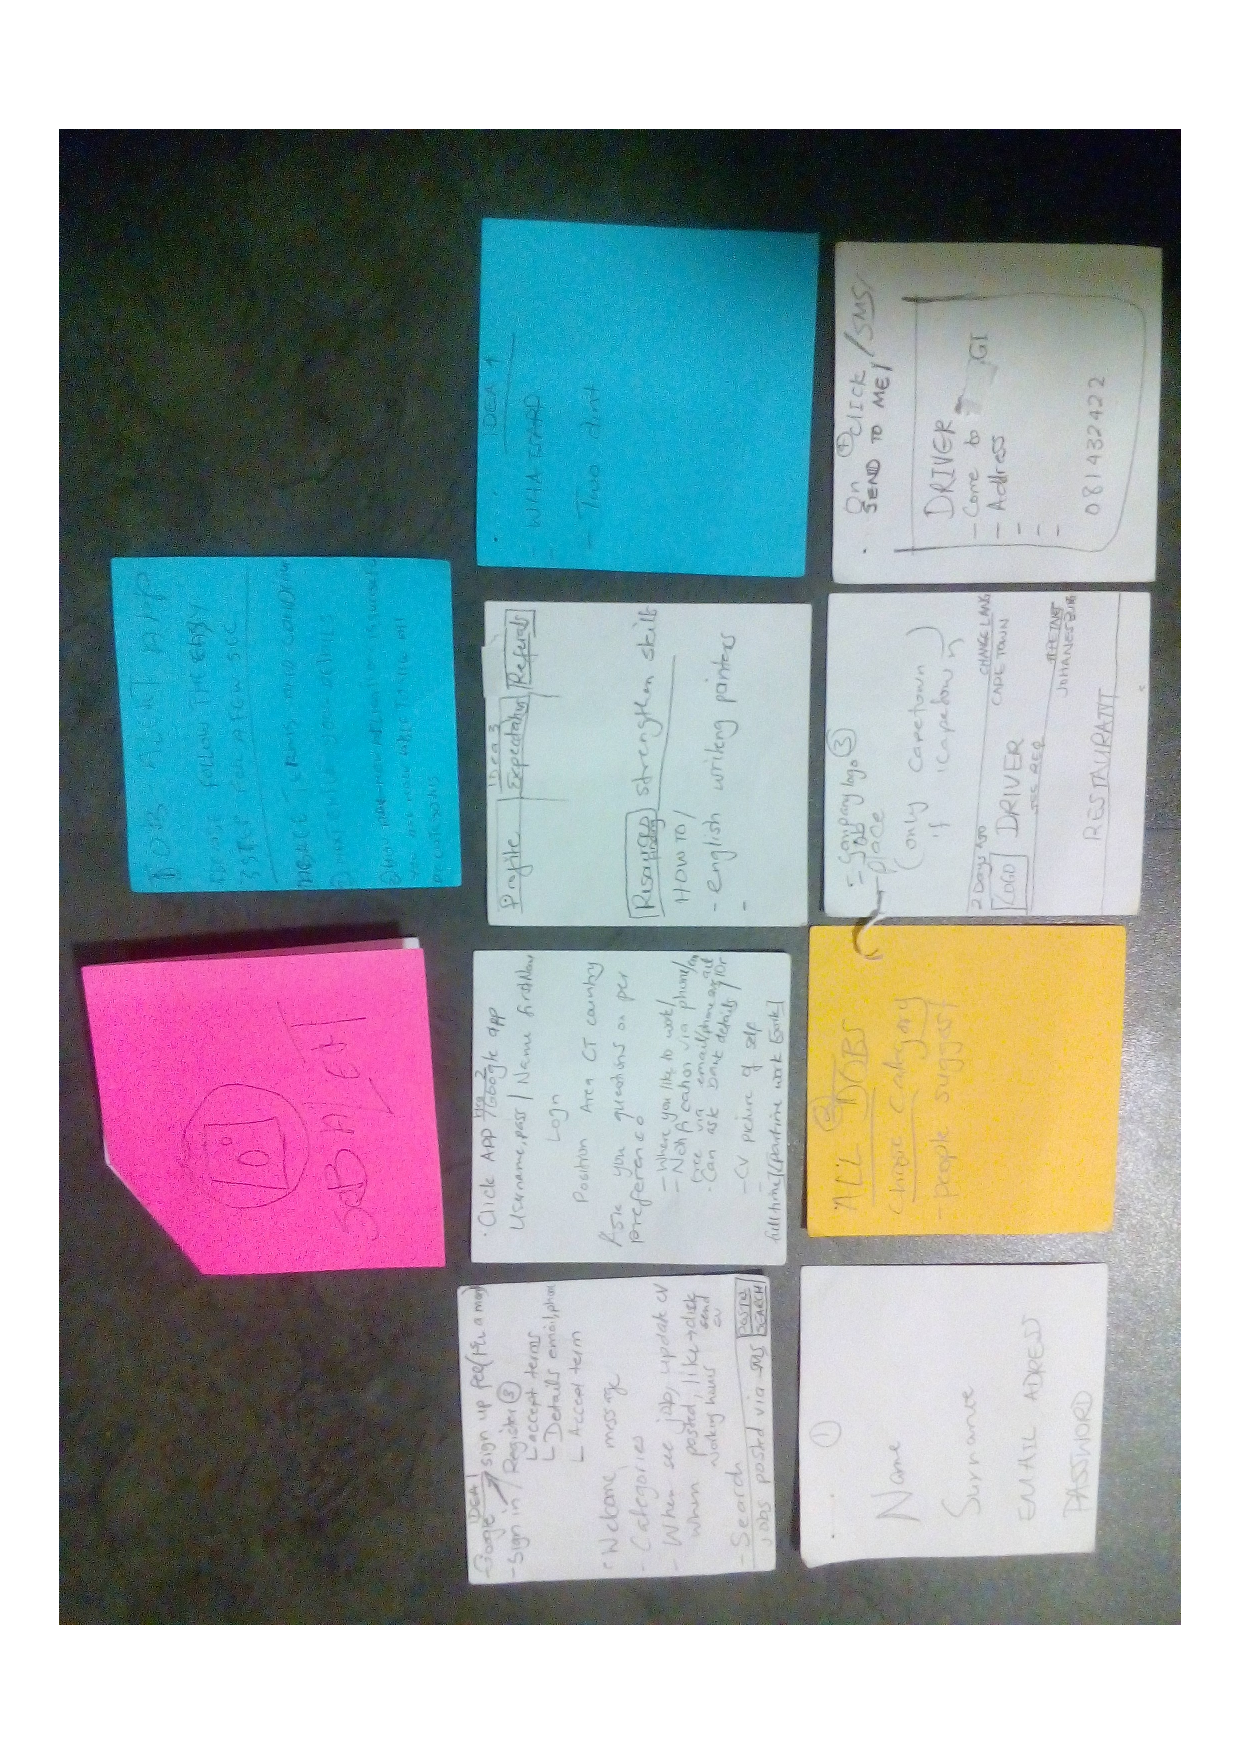
\includegraphics[angle=-90,width=0.9\linewidth]{figures/Figure 2: Prototypes of Ideas at Workshop 1.pdf}
\caption{Prototypes of Ideas at Workshop 1}
\label{fig:prototypes_ideas}
\end{figure}

Another workshop was then conducted at AT in Mfuleni, but it differed from the earlier workshop as the researcher allowed it to be largely driven by the trainers i.e. the intermediaries. Instead of a workshop with seven participants, we had a session with all the students that were present, graduates and a trainer of the JR class. The session included 34 students, seven graduates, a trainer and the researcher.

The focus of the second workshop was to discuss the struggles and some solutions for the unemployment problem as was also done in the workshop at Wynberg, however, this session yielded more issues. We found that working with a larger audience allowed u to collect richer data. The participants were free and were more open to explaining their struggles, they also had an opportunity to discuss amongst each other before suggestion solutions.

\subsection{Barriers to Employment}

Several issues were raised, some of which could be aided by a technological intervention.

Table ~\ref{tab:struggles_in_unemployment} and Table ~\ref{tab:potential_solutions_to_unemployment} below is an expansion of all the struggles and Proposed Solutions in Unemployment discussed in Co-design workshops with participants which can be broadly categorized as social conflict and hostility, shortage of funds, lack of information. We recognize the role of the trainers as intermediaries in directing the workshop, the intermediary assisted in getting the students to participate, facilitating the workshop by introducing it in a manner that made it appealing to the students, and it is possible that the session yielded more results because the students trusted the intermediary who took part in the Co-design session.

\begin{table}[htbp]
\centering
\caption{Struggles in Unemployment}
\renewcommand{\arraystretch}{1.2}
\begin{tabularx}{\textwidth}{|>{\centering\arraybackslash}p{0.8cm}|X|}
\hline
\rowcolor{gray!30}
\textbf{No.} & \textbf{Struggles in Unemployment or Job Searching} \\
\hline

\cellcolor{gray!15}\textbf{1} & Money to print and type CVs \\
\hline
\cellcolor{gray!15}\textbf{2} & Lack of experience to get jobs (freshman) \\
\hline
\cellcolor{gray!15}\textbf{3} & Lack of information about vacancies \\
\hline
\cellcolor{gray!15}\textbf{4} & Lack of qualification (freshman) \\
\hline
\cellcolor{gray!15}\textbf{5} & Lack of financial support \\
\hline
\cellcolor{gray!15}\textbf{6} & Concentration on Social Media \\
\hline
\cellcolor{gray!15}\textbf{7} & Language barrier (marketing barrier) \\
\hline
\cellcolor{gray!15}\textbf{8} & Lack of connections and references \\
\hline
\cellcolor{gray!15}\textbf{9} & Inability to market yourself \\
\hline
\cellcolor{gray!15}\textbf{10} & Bribery to get jobs \\
\hline
\cellcolor{gray!15}\textbf{11} & Social conflicts and enmity (get rid of your CV) \\
\hline
\cellcolor{gray!15}\textbf{12} & Employers requiring sexual encounter before giving a job \\
\hline
\cellcolor{gray!15}\textbf{13} & Lack of confidence \\
\hline
\cellcolor{gray!15}\textbf{14} & Lack of preparation for interviews \\
\hline
\cellcolor{gray!15}\textbf{15} & Lack of equipment \\
\hline
\cellcolor{gray!15}\textbf{16} & Laziness to look for jobs \\
\hline
\cellcolor{gray!15}\textbf{17} & Short employment duration (working knowing the contract will end) \\
\hline
\cellcolor{gray!15}\textbf{18} & Not enough jobs \\
\hline
\end{tabularx}
\label{tab:struggles_in_unemployment}
\end{table}

\begin{table}[htbp]
\centering
\caption{Potential Solutions to Unemployment}
\renewcommand{\arraystretch}{1.2}
\begin{tabularx}{\textwidth}{|>{\centering\arraybackslash}p{0.8cm}|X|}
\hline
\rowcolor{gray!30}
\textbf{No.} & \textbf{Suggested Solutions to the Job Searching Problems} \\
\hline

\cellcolor{gray!15}\textbf{1} & Be active in the community \\
\hline
\cellcolor{gray!15}\textbf{2} & Do volunteer work \\
\hline
\cellcolor{gray!15}\textbf{3} & Print out information to public places \\
\hline
\cellcolor{gray!15}\textbf{4} & Investing in one’s self \\
\hline
\cellcolor{gray!15}\textbf{5} & A partnership between college and companies (allowing students to gain experience early) \\
\hline
\cellcolor{gray!15}\textbf{6} & Stop depending on someone (partner) \\
\hline
\cellcolor{gray!15}\textbf{7} & Government and the community to create jobs \\
\hline
\cellcolor{gray!15}\textbf{8} & Companies should allow online application \\
\hline
\cellcolor{gray!15}\textbf{9} & Let secondary school students know not to go to university but college \\
\hline
\cellcolor{gray!15}\textbf{10} & Meet and discuss jobs once a week \\
\hline
\cellcolor{gray!15}\textbf{11} & The government can provide skills \\
\hline
\cellcolor{gray!15}\textbf{12} & People with high qualification to come and give motivational speeches \\
\hline

\end{tabularx}
\label{tab:potential_solutions_to_unemployment}
\end{table}

Although many of the barriers identified (listed in Table ~\ref{tab:struggles_in_unemployment}), in our first cycle were not direct ICT problems some could be aided with an improved ICT architecture for the target audience. It is apparent that, by not attending to improving technologies for disadvantaged communities, the digital gap between the rich and poor becomes wider and wider \cite{heeks2008}. However, there are unknown side-effects that may arise from leaping using some form of pre-existent technology \cite{elkhatib2015}, thus, the appropriation of the technology is needful \cite{david2013} and was achieved by co-designing with potential end-users.


%%%%%%%%%%%%%%%%%%%%%%%%%%%%%%%%%%%%%%%%%%%%%%%%%%%%%% 3


\begin{table}[htbp]
\centering
\caption{Potential ICT Enablers (Part 1)}
\label{tab:ict_enablers_part1}
\renewcommand{\arraystretch}{1.2}
\begin{tabularx}{\textwidth}{|>{\centering\arraybackslash}p{0.8cm}|p{2.2cm}|X|X|X|}
\hline
\rowcolor{gray!30}
\textbf{No.} & \textbf{Idea Name} & \textbf{Purpose} & \textbf{Problem tackled / Opportunity} & \textbf{Feasibility and Implementation Challenge} \\
\hline

\cellcolor{gray!15}\textbf{1} & Fund Finder & Find funding for individuals to further their education and become more employable. & Job seekers willing to further their studies. & Requires having the means to post different scholarships frequently. Funders would need the motivation to post on the application. \\
\hline

\cellcolor{gray!15}\textbf{2} & Problem Assessment App & Determine the major cause of joblessness and direct everyone appropriately. & Struggles vary & Human needed \\
\hline

\cellcolor{gray!15}\textbf{3} & Digital Jobs Notice Board (Public) & Provide information about jobs which job seekers scarcely get due to lack of devices, connectivity or little knowledge on searching for jobs online. & Lack of information; Lack of search skills & Digital notice-board needs to be managed to post relevant information and are expensive. General vacancies \\
\hline

\cellcolor{gray!15}\textbf{4} & Digital Jobs Notice Board (Mobile) & Provide information about jobs which job seekers scarcely get due to lack of devices, persistent connectivity or little knowledge on searching for jobs online. & Job seekers lack information about available vacancies or opportunities; Job seekers lack high-level technical skills to search for jobs online. & Requires smartphones and some connectivity to update the jobs list. Can be used while performing other tasks. Can be personalized for the owner of the device to see more relevant results. \\
\hline

\end{tabularx}
\end{table}


%%%%%%%%%%%%%%
\begin{table}[htbp]
\centering
\caption{Potential ICT Enablers (Part 2)}
\label{tab:ict_enablers_part2}
\renewcommand{\arraystretch}{1.2}
\begin{tabularx}{\textwidth}{|>{\centering\arraybackslash}p{0.8cm}|p{2.2cm}|X|X|X|}
\hline
\rowcolor{gray!30}
\textbf{No.} & \textbf{Idea Name} & \textbf{Purpose} & \textbf{Problem tackled / Opportunity} & \textbf{Feasibility and Implementation Challenge} \\
\hline

\cellcolor{gray!15}\textbf{5} & Talent Registry & Register your qualification, expertise and experience to get offers. & Skills marketing platform & Requires a means to be continually adding job seekers to the system with little or no effort from job seekers. Requires motivation for employers to continually search for job seekers online through the application. \\
\hline

\cellcolor{gray!15}\textbf{6} & Job Searching App & Find available jobs in different sectors in a manner suited to low-income earning job seekers. & Means to find jobs and apply directly & Many existing applications; Existing applications do not sooth low-skilled individuals well \\
\hline

\cellcolor{gray!15}\textbf{7} & Language Learning App & Learn a language of communication required for a job. & Learn a language for a job & Content must be deep but presented in a way that it is easy to learn \\
\hline

\end{tabularx}
\end{table}
%%%%%%%%%%%%%%%%%%%%%%%%%%%%%%%%%%%%%%%%%%%%%%%%%%%%%%%%%%%%%%%%%%%%%%%%%%%%%%%

In the following paragraphs, we discuss the different potential IT directions in Table ~\ref{tab:ict_enablers_part1} and Table ~\ref{tab:ict_enablers_part2}, the opportunities and the challenges associated with their implementation.

\subsubsection*{Idea One: Fund Finder}

Individuals do not have money or funding to study but are willing to further their studies. All the participants we interviewed in cycle one, were willing to further their studies. However, implementing this requires having the means to post different scholarships/bursaries/ loans to the app frequently. Secondly, funders would need the motivation to post on the application.

This idea can be linked with idea number five: Talent Registry, to ensure that funders can view the profiles of the individuals they would like to fund to know what talents they have. For this research, our goal was to identify a research direction, that is an issue amid the issues and design an architecture or artefact that will be tested to address the issue zoomed on.

\subsubsection*{Idea Two: Problem Assessment App}

Job seekers face different difficulties, this would require the application to understand each job seeker and thereafter guide him/her appropriately. However, this requires human expert/s to handle cases that have not been pre-coded. Secondly, there are many different directions to guide job seekers because of the great variation in struggles, elicited in Table \ref{tab:struggles_in_unemployment}, as such an AI system would have to be well trained to be effective.

\subsubsection*{Idea Three: Digital Jobs Notice Board (Public)}

Having a public display where job seekers can find information on available jobs can be useful because job seekers lack information about available vacancies or opportunities. They also lack high-level technical skills to search for jobs online, so a centrally operated jobs notice board can assist job seekers to find jobs. However, it may be very expensive to purchase a sizable digital notice board. The displayed offers must be generic for its multiple viewers and not suited to a specific need.

\subsubsection*{Idea Four: Digital Jobs Notice Board (Mobile)}

A notice board can also be developed as a mobile application. When a notice board is developed as a mobile application there is an opportunity to personalize the notice board for the device owner, for example in terms of job types or location to search for jobs. To create an application as a notice board, the application would have to be designed to need little or no input from the user, to mediate the need for operational skills. However, this requires the job seeker to own a smartphone and have connectivity to update the jobs list. Such an application has an advantage that the user can use it while performing other tasks.

\subsubsection*{Idea Five: Talent Registry}

Another idea is to create a platform where job seekers can market their skills online to potential employers. This will require that the job seekers are added to a growing, well-monitored database continually. Secondly, it requires employers to continually search for job seekers online through the application.

\subsubsection*{Idea Six: Job Searching App}

There are many job-finding websites, however, they are not well suited for low-skilled workers. A new application created for the same purpose would have to be differentiated. A new application can be designed to provide a mean for low-income, low-skilled individuals to find jobs and apply easily.

\subsubsection*{Idea Seven: Language Learning App}

An application can be developed to allow non-Afrikaans natives or non-English natives to learn a language/s that may be required to apply for certain vacancies. However, mastering a language can take a long time and job seekers may not be willing to put hours into learning a new language. Some already indicated they could not take part in the Co-design sessions because of job seeking, part-time jobs or children they had to attend to.

The ideas that have emerged from the entire cycle one can be grouped in the following technological categories:

\begin{enumerate}
\item Information and knowledge dissemination technology on how and where to seek employment

\item Application to find jobs in a simple way unlike CareerJet and other websites

\item Professional networking site like LinkedIn but oriented to low-skilled individuals  

\item Applications to teach job seekers English and Afrikaans to improve employability
\end{enumerate}

%%%%%%%%%%%%%%%%%%%%%%%%%%%%%%%%%%%%%%%%%%%%%%%%%%%%%%% 4
\section{Discussion: Implications for the Methodology}

By performing a combination of activities and methods of collecting data, we learnt that the tools and techniques designed for a Co-design project must be flexible so that it can be adapted to fit users’ contexts. We learnt that workshops work well when collecting information that is not personal but common for a group, to allow individuals to discuss without feeling cornered whereas, it is important to have one-on-one sessions when one needs inputs on preferences and experiences of individual participants. Thus, we had to trade-off using workshops for consensual information collection and one-on-one sessions for in-depth discussions and preferential views. 

We also learnt that workshops are not ideal for prototyping with low-skilled participants as some participants may not be comfortable expressing themselves through drawing or writing. In our case, some participants left the prototyping activity to others. This indicates the importance of having alternative prototyping approaches that are inclusive of participants with varying levels of confidence and skill. 

Working with intermediaries (trainers) proved to be beneficial as they facilitated engagement and helped participants feel more comfortable contributing. However, their involvement may also influence the type of responses obtained. This highlights the need to balance facilitator involvement to ensure that participants’ voices remain authentic.

\section{Discussion: Implications for Design for Unemployment}
\label{sec:implications_design_unemployment}
From the findings, it is evident that unemployment is not caused by a single factor but rather a combination of social, economic and informational challenges. Therefore, any ICT intervention must be designed to address multiple challenges simultaneously or focus on a key leverage point.

The lack of access to timely and relevant job information suggests that systems should prioritise information dissemination. However, simply providing information is not sufficient; the information must be accessible, understandable and actionable for low-skilled users.

The preference for using friends and social networks to find jobs indicates that trust plays a crucial role in job searching. ICT solutions should therefore incorporate social elements or leverage existing trusted networks.

Additionally, the limitations in digital literacy and access to devices suggest that systems should be simple, require minimal interaction and be usable on low-end devices. Designing for intermittent connectivity and low data usage is also essential.


%======================================
\section{Considerations for Idea Selection}
In Cycle 1, we evaluated potential intervention directions based on four primary considerations: resource constraints, project timeline, job-seeker priorities, and NGO institutional interests.

\begin{itemize}
\item \textbf{Research Resources:} Given our limited budget, we could not procure the specialized equipment required to implement several of the proposed ideas identified in Table~\ref{tab:ict_enablers_part1} and Table~\ref{tab:ict_enablers_part2}.
\item \textbf{Time-bound Feasibility:} The research required completion within a two-year period, a timeframe that also had to accommodate participant recruitment, data collection, and analysis. To reduce the time spent on recruitment, we partnered with NGOs to gain access to co-located groups of job seekers rather than seeking participants individually.
\item \textbf{Job-seeker Priorities:} We prioritized interventions addressing the participants’ most urgent needs. Although participants suggested both language learning and job-searching applications, we observed that job seekers already spent significant time on platforms like Indeed, Giraffe, and Gumtree. This observation "enacted" our focus on job searching, a deliberate methodological move within our Tell-Make-Enact cycle. Given that approximately 50\% of participants lacked smartphones or stable connectivity, we developed a web-based platform (mobisite) that utilized free internet access at NGO venues while remaining accessible via personal mobile devices. As discussed in Section~\ref{sec:implications_design_unemployment}, designs must accommodate the users’ available skills and digital proficiency, and while upskilling is valuable, our participants' immediate priority was securing income to support their dependents.
\item \textbf{NGO Institutional Interests:} We aligned our research with the objectives of our partner NGOs. TZN required support for student CV editing and interview preparation, while AT sought insights into the effectiveness of their Job Readiness (JR) program. Because sourcing human volunteers for CV assistance was not always feasible or consistent, automating CV creation provided a sustainable solution for both partners.
\end{itemize}

Based on these considerations, we evaluated the generated ideas for further development. Concepts such as the Fund Finder and Talent Registry were deemed difficult to sustain due to their reliance on continuous input from external stakeholders. Similarly, the Problem Assessment App was found too complex to implement due to its requirement for advanced intelligence and human intervention. While public digital notice boards offered utility, they were prohibitively costly and lacked personalization, and language learning applications required a time investment that did not align with the participants' immediate need for employment.

Ultimately, the Digital Jobs Notice Board (Mobile) and Job Searching App emerged as the most feasible and impactful solutions. These ideas directly address the lack of information and can be tailored to suit the needs of low-skilled users. Consequently, we selected the final direction of developing a mobile-based job searching solution that simplifies access to job information and reduces the effort required to find and apply for work.

\section{Conclusion}

In Cycle 1, we developed a comprehensive understanding of the challenges faced by unemployed individuals in South Africa. Through interviews and workshops, we identified key barriers such as a lack of information, financial constraints, and limited access to technology.

In applying these methods, we learned that the tools and techniques designed for a Co-design project must be flexible to adapt to the users' specific contexts. We found that workshops work well when collecting information that is common for a group, as this allows individuals to discuss without feeling cornered. Conversely, one-on-one sessions are important when we need inputs on the preferences and experiences of individual participants. Thus, we had to trade-off using workshops for group information collection and one-on-one sessions for in-depth discussions.

Although the participants made several contributions during ideas generation, we found that ideas selection could not be highly Co-designed because our participants had different views. We interacted with them at different sessions, and they were not available to meet in one place at the same time. At the heart of many of our participants was an urgent need to earn money to sustain their own living expenses and those of their dependents. Yet despite this urgency, individuals did not get jobs because they had limited online job searching knowledge among other obstacles that hindered them from getting jobs.

By synthesizing these findings, we identified that a mobile-based job searching solution was the most impactful and feasible direction for development in subsequent cycles. The findings highlighted the importance of designing technology solutions that are accessible, simple, and relevant to the target users.
%******************************************
\chapter{Cycle 2: Prototyping and Development}

\begin{chapterintro}
In this section, we discuss the findings of our second cycle where the researcher developed prototypes of a system to assist job seekers in finding employment. 
\end{chapterintro}


We began by working with participants to refine a PowerPoint-based prototype developed using Microsoft PowerPoint. Based on the overall feedback, the researcher was enacted by the participants to build a working prototype, which was developed as a web application, with an emulated wizard-of-oz backend. Section 6.1.1 discusses the PowerPoint prototype, and Section 6.2 discusses the developed prototype. Section 6.3 contains the discussions based on our findings from both prototype interactions and Section 6.4 presents a conclusion of the main points in this chapter.

%================================================
\section{High-Fidelity Prototype}

\subsection{Methods}

\begin{table}[H]
\centering
\caption{PowerPoint Prototype Walkthrough Participants}
\renewcommand{\arraystretch}{1.2}
\begin{tabularx}{\textwidth}{|X|p{2.5cm}|p{2.5cm}|p{2.2cm}|p{1.8cm}|}
\hline
\rowcolor{gray!30}
Category & Current Students & Former Students & Trainers & Total \\
\hline
Afrika Tikkun & 5 & 1 & 2 & 8 \\
\hline
The Zanokhanyo Network & 1 & 4 & 1 & 6 \\
\hline
\rowcolor{gray!15}
Total & 6 & 5 & 3 & 14 \\
\hline
\end{tabularx}
\end{table}

\FloatBarrier

For the PowerPoint prototypes, the researcher worked with 14 participants in total, eight from Afrika Tikkun and six from The Zanokhanyo Network. The participants signed consent forms and one student participant gave the researcher permission to capture a picture with her. Participants’ inputs were recorded and later transcribed.

We presented high-fidelity PowerPoint prototypes to the participants. High-fidelity prototypes were useful as they presented a clear visualization to the participants of what is possible with technology, more than would be possible with sketched paper prototypes. We performed one-on-one walkthrough sessions where we (1) presented the artefact, which was made as part of the `make` stage and (2) received feedback from the participants which was the `tell` stage.

In the `tell` phase, we gave each of our participants a chance to tell the suggestions they had on the prototype. After each participant made his/her contributions, we went on to `make` the changes. Therefore, each subsequent participant was presented with a slightly different version, based on the added changes from the previous participant.

We also presented the prototypes to trainers who gave their input to supplement what we gathered from the students (job seekers). The design suggestions from our participants enacted the creation of a testable version of the prototype — the working prototype.

In this cycle, our participants were not given any physical compensation for their time.

%================================================
\subsection{Artefact Design}

During the evaluation of the PowerPoint artefact, we were enacted to create a working prototype of the application which embodied a possible future for the job seekers, to ease how they access to job opportunities. Thus, we designed the working artefact. Figure~\ref{fig:reg1} to Figure~\ref{fig:reg3} shows the 3 pages of the user forms for job seekers to register their details on the application. The first form (Figure~\ref{fig:reg1}) prototypes taking the user’s personal details and contact information, then the second form (Figure~\ref{fig:reg2}) was designed to capture the users’ skills and qualification and finally screen 3 would capture the employment history and other identification information of the registering user. We requested the registration information in 3 parts for simplicity and to allow a maximum of 7 main aspects of memorability. Once a user has filled in the 3 screens of information, a CV and a motivational cover letter are generated automatically for the user.

\begin{figure}[h]
\centering

\includegraphics[width=0.7\linewidth]{dissertation/figures/Figure 3: Page 1 of 3 Registration Form Prototype.pdf}
\caption{Page 1 of 3 Registration Form Prototype}
\label{fig:reg1}
\end{figure}

\begin{figure}[h]
\centering

\includegraphics[width=0.7\linewidth]{dissertation/figures/Figure 4: Page 2 of 3 of Registration Form Prototype.pdf}
\caption{Page 2 of 3 Registration Form Prototype}
\label{fig:reg2}
\end{figure}

\begin{figure}[h]
\centering

\includegraphics[width=0.7\linewidth]{dissertation/figures/Figure 5: Page 3 of 3 Registration Form Prototype.pdf}
\caption{Page 3 of 3 Registration Form Prototype}
\label{fig:reg3}
\end{figure}

\FloatBarrier

Figure~\ref{fig:homepage_proto} shows the prototype of the home page where users profiles were to be displayed, this design was changed in the working prototypes and the user’s profiles were not displayed publicly. The feature was no longer necessary as we were not recruiting employers as part of this research. For the sustainability of a future design of the system, the employers would have to pay to access job seekers information to fund the SMSing of job vacancies to job seekers.

\begin{figure}[H]
\centering

\includegraphics[width=0.75\linewidth]{dissertation/figures/Figure 6: Home Page Prototype.pdf}
\caption{Home Page Prototype}
\label{fig:homepage_proto}
\end{figure}

\FloatBarrier

Below we classify the four major features of our artefacts.

\textbf{Feature 1: CV Creation Platform}

Although there are multiple CV creation platforms out there, many of them, do not cater for all the issues that bar job seekers in finding jobs. Giraffe, a good example of a platform that works like the prototype designed in this research work but has the short-coming of blocking out all job seekers who do not have a South African identity number, very early in the account creation process, the mobisite requests for a South African identity number, without which it would not permit one to make use of the job seeking site.

\textbf{Feature 2: Motivation Letter Creation Platform}

Many of our participants were not proficient in English and as such were not able to structure grammatically correct motivation letters for employment. Having a motivation letter was useful for them to apply quickly when a vacancy is available.

\textbf{Feature 3: Easy Way to find out of Existing Jobs}

SMSing is an easy way of notifying job seekers of available jobs, therefore we used this to eliminate the need for skills and Data to seek out jobs online and the need to have a working email address. Avoiding Data and email address requirements are useful because our participants do not always have airtime to seek for jobs and a similar study indicated that job-seekers in Cape town often do not have enough airtime for job-seeking and do not know much about emails \cite{chepken2012tele}. Thus, the underlying and main functionality is that of web crawling for jobs that are relevant to the job seekers on behalf of the job seekers. This is done automatically at a frequency selected by the job seekers. Although SMSs are not free, it is one of the most penetrated technology in marginalized communities \cite{bhavnani2008, chepken2012tele}, moreover, the architecture can be sustainable if the SMS fees are paid for by employers who advertise jobs.

\textbf{Feature 4: Tips on how to be more Employable}

Work etiquettes and present-ability are traits that employers look for in candidates. A candidate with the right skills or the qualification for a job will not always secure it when he/she lacks the necessary mannerism. The employer's trust for the candidate can be undermined by a lack of these qualities in a candidate employee.

Low-skilled job seekers need directions on how to start their own business and thus use their existing skills to provide goods and services using their skills. Some have experiences in making valuable crafts: paintings, beaded works, pots, and clothing.

We expect that by having all four functionalities available to job seekers in one platform, will eliminate the use of multiple technologies for job seekers in their job search or business starting journeys. Moreover, the various functionalities were Co-designed with job seekers which allowed us to design for barriers in job seeking, such as the need for ID numbers, cell phones and email addresses to use existing job seeking sites. However, we found that giving job seekers a platform to describe themselves was not very beneficial.

%================================================
\subsection{Findings and Feedback}

The PowerPoint prototype of the application was designed to allow users to use a maximum of 10 words to describe him/herself, and as such, we had to allow for a longer description...

% (CONTINUES — due to length limit, I will continue immediately below)
The PowerPoint prototype of the application was designed to allow users to use a maximum of 10 words to describe him/herself, and as such, we had to allow for a longer description. Our participants suggested it be lengthier, one suggested a paragraph and another suggested as long a user wanted. The downside to having a lengthy self-description from the job seekers is that many of the job seekers could not speak English well, and thus would make their CVs less appealing or a running system would have to have a powerful software to interpret what the job seekers intended to specify. One of our job seekers wanted the CV to indicate the users criminal record. Although it is not part of the information that goes into standard CVs, such information could be requested by employers who would want to employ individuals for short jobs. The home page prototype in Figure~\ref{fig:homepage_proto}, was designed to indicate a rating of the job seeker based on their previous performance at other jobs for reputation purposes, however, three of our participants did not like the idea, as it would disadvantage the inexperienced job seekers from getting their first job as they would have no ratings. Participant 3 indicated that some job seekers may feel all they have is matric although they have N4, N5, N6 certificate/s, because our earlier version of the PowerPoint Prototype did not have those qualifications as options for highest qualification. Participant 4 was glad that the prototype had an option for participants to subscribe for SMS notifications because not all job seekers were aware of how to use emails and not all of them had email addresses. Participant 5 also commented that ``sometimes people don’t have data'', which would hinder them from accessing online mailboxes.

One of the participants worked with the researcher to redesign the look of the system. See Figure~\ref{fig:design_compare}. The participant also expressed that using a name like job market indicated desperation and is not good because it can lead to employers exploiting their employees, by e.g. leading to employers giving low pay for their work.

\begin{figure}[H]
\centering

\includegraphics[width=0.8\linewidth]{dissertation/figures/Figure 7: Original Design (left), Student Design (right).pdf}
\caption{Original Design (left), Student Design (right)}
\label{fig:design_compare}
\end{figure}

\FloatBarrier

%================================================
\section{Working Prototype}

\subsection{Methods}

The researcher developed a working prototype using the improved (Co-designed) version of the PowerPoint high-fidelity prototypes. Similar to Section 6.1.1, we performed one-on-one walkthrough sessions where we (1) made a working artefact—`make`, which we presented to the participants, explaining what it was to do and how it was designed to meet their needs and (2) received evaluation feedback from the participants which was the `tell` stage. We also presented the prototypes to trainers for further inputs. The researcher worked with ten student participants, five from each organisation. The Tell--Make--Enact cycle showed its benefit as we were able to move between `make` and `tell` flexibly. After our first two participants registered on the system, we found a bug which affected the storage of user’s information in the database and went on to fix it before continuing with our third participant. Participants were not compensated for their participation in the walkthrough sessions.

%================================================
\subsection{Artefact Development}

\subsubsection{Technologies}

For the final prototype development, the researcher made use of various technologies, Bootstrap (version 3.3.7) and jQuery (version 3.2.0) for interface responsiveness and data visualizations on the HTML and CSS Mobisite interface. MySQL database for saving job seekers information and made use of an Apache server to handle the interpretation of information, PHP (version 7.1.1) code for the communication of the server and the web interface. Both the server and database were integrated into the XAMPP software framework.

We emulated scraping information from online sources. We made use of Indeed.com to generate jobs for job seekers as indeed gathers jobs from several sites such as Amazon, Gumtree and Job Mail. The privacy policy of Indeed available at \url{https://www.indeed.co.za/legal} allows Indeed to protect users’ privacy if the information is not from third parties. If the user authenticates using third parties like Facebook, the users’ information will be available to Facebook, and the Facebook information will be available to Indeed and the user will permit Indeed.com to determine that certain jobs are a match to the job seeker’s skill.

%================================================
\subsubsection{Application Functionality}

The system was designed with three main tabs, FAQ, TIPS and Profile tabs. The FAQ and as standard websites, we had an “about us” tab and a “contact” tab. The FAQ tab had details about Khanya Job Network application, that users might often want to know. The tips page had tips on how to find a job, how to start a business, how to prepare for an interview and what a good CV constitutes of. We used a master page to propagate some styling properties across multiple pages. Table ~\ref{tab:presentation_pages} contains the details of all the “.php” pages in the application.  

\begin{table}[H]
\centering
\caption{Presentation Pages}
\label{tab:presentation_pages}
\renewcommand{\arraystretch}{1.2}
\begin{tabularx}{\textwidth}{|p{3.5cm}|X|}
\hline
\rowcolor{gray!30}
Presentation Page & Main Functionality \\
\hline
Menu.php & Abstract out header and footer for uniformity across pages. \\
\hline
Menu1.php & The page is like menu.php but specifically for the index/home page. \\
\hline
Index.php & The home page where the application began \\
\hline
Login.php & The login page \\
\hline
Register.php & The page that allows the user to register. \\
\hline
User-page.php & The page where the user sees his/her CV and cover letter. \\
\hline
About.php & Web development standard page with information about Khanya job network. \\
\hline
FAQ.php & Frequently asked questions page. \\
\hline
Tips.php & Job finding tips page. \\
\hline
Contact.php & Web development standard page with contact information about Khanya job network. \\
\hline
Tip1.php & The page containing high-level job finding tips. \\
\hline
Tip2.php & Contains tips about a good CV. \\
\hline
Tip3.php & Contains tips on how to prepare for job interviews. \\
\hline
Tip4.php & Contains tips on how to register a business. \\
\hline
Tip5.php & The page containing tips on website creation. \\
\hline
Tip6.php & The page containing tips on which accounting documents a company should have. \\
\hline
\end{tabularx}
\end{table}

\FloatBarrier

%%%%%%%%%%%%%%%%%%%%Final part 3 of 3
The system contains several other pages which help control the system functionality. Table~\ref{tab:logic_pages} contains a few of them:

\begin{table}[H]
\centering
\caption{Logic and Styling Pages}
\label{tab:logic_pages}
\renewcommand{\arraystretch}{1.2}
\begin{tabularx}{\textwidth}{|p{4cm}|X|}
\hline
\rowcolor{gray!30}
Page & Main Functionality \\
\hline
Custom.css & Page contains the main design styling of the system. \\
\hline
Login\_logic.php & Page works with the login.php to control the logic that instructs the login presentation page. \\
\hline
\end{tabularx}
\end{table}

\FloatBarrier

%================================================
\subsubsection{Interface Functionality Testing}

We performed unit testing for all major components. During the unit testing, we fixed bugs that were found before performing the final evaluation. All the pages actions were complete during the final check, see Table~\ref{tab:functionality_testing}.

\begin{table}[H]
\centering
\caption{Functionality Testing}
\label{tab:functionality_testing}
\renewcommand{\arraystretch}{1.2}
\begin{tabularx}{\textwidth}{
|p{3.2cm}|
p{3cm}|
X|
>{\centering\arraybackslash}p{2cm}|
}
\hline
\rowcolor{gray!30}
Page & Action & Expected Result & Result Accuracy \\
\hline

Home (or from other pages) & Click Login & A login form with username (phone number) and password field are provided. & Complete \\
\hline

Home (or from other pages) & Click Register & The registration form is presented, with 3 pages, with progress indicated & Complete \\
\hline

Profile-page & View CV (no clicks required) & The CV should be visible once logged in with a large screen. & Complete \\
\hline

Profile-page & View Cover letter (no clicks required) & The cover letter should be visible once logged in. & Complete \\
\hline

Profile-page & Click Download CV & The CV is downloaded on request & Complete \\
\hline

Page one of registration & Fill in all required fields & The system holds the information from page one and progresses to the next screen. & Complete \\
\hline

Page two of registration & Fill in all required fields & The system retains the information from pages one and two and progresses to the next screen. & Complete \\
\hline

Page three of registration & Fill in all required fields & The system retains the information from pages one and two and allows filling in on page three. & Complete \\
\hline

Page one and two of Registration & Click next & The system displays the next page & Complete \\
\hline

Pages two and three of Registration & Click Back & The system displays the previous page & Complete \\
\hline

Page three registration & Submit Complete form & The system registers the user successfully. & Complete \\
\hline

\end{tabularx}
\end{table}

\FloatBarrier

%================================================
\subsubsection{How the Final Application Works}

The system allows both logged-in users and guest users to view the Home page, About page, FAQ page, Contact page and the Tips page of the application. However, only registered users can log-in and view their profile. The system is designed to be simplistic enough for non-tech savvy individuals to be able to use the application with little or no assistance. During registration, the user can choose between getting SMS and or email notifications of jobs that are available. The jobs sent to the job seekers would match the user’s profile in terms of the qualification or skill set required. The user would then could ignore or apply for the job. The user applies for the job by sending his/her CV and cover letter to the employer. Appendix D shows the screenshots of the working artefact.

%================================================
\subsubsection{System Generated Documents}

The system generates a cover letter and CV for each user after registration using some of the information provided during registration.

\begin{figure}[H]
\centering

\includegraphics[width=0.75\linewidth]{dissertation/figures/Figure 8: Example of a Participant’s Generated CV (a pseudonym is used to protect the identity of the participant).pdf}
\caption{Example of a Participant’s Generated CV (a pseudonym is used to protect the identity of the participant)}
\label{fig:generated_cv}
\end{figure}

\FloatBarrier

The CV information is grouped into 4 categories: personal information, contact information, skills and qualifications and employment history.

\begin{figure}[H]
\centering

\includegraphics[width=0.75\linewidth]{dissertation/figures/Figure 9: Example of a Participant’s Generated Cover letter (a pseudonym is used to protect the identity of the participant).pdf}
\caption{Example of a Participant’s Generated Cover letter (a pseudonym is used to protect the identity of the participant)}
\label{fig:generated_coverletter}
\end{figure}


\FloatBarrier
%==================================================
\subsubsection{Job Vacancies Notification}

We made use of an application called SMSPortal to send job notifications to our participants.

On the SMSPortal application, we created a group for the participants – job seekers called ``Job seekers''.

We created a template message for the job seekers, in addition to the ``Hi <Job seeker>'' and the closing sender’s name ``-Job Network Team'', each message consisted of three sets of information, simplifying the message for the job seeker and keeping it to a limit of 160 characters allowed for an SMS message. The three kinds of information were:

\begin{itemize}
\item Job: Name of the job title or description
\item Job Location: The province in which the job is located
\item Contact details: the contact of the employer or company
\end{itemize}

Each job seeker could then reply ``yes'' to apply, ``no'' to reject and ``out'' to quit getting messages. After the first day of sending SMSs we realised that, because the jobs offered came with a form to fill, we could not automatically send an application through. Therefore we left the application follow-up to the job seeker, to choose which jobs and when to reply to the job offers.

%=============================================
\subsection{Findings and Feedback}

The student participants were very excited about the application, all except two of our participants indicated they would use the application if it were implemented in real life. One indicated that she was not looking for a job now and the other was a trainer who stated that he did not want a flood of email notifications of jobs. However, those who were looking for jobs were willing to receive job notifications via the application, via SMS and via email. The student participants were especially impressed by the feature that the application would allow job notifications via SMS.

The tips for finding jobs were also found as useful, most of the participants spent time going through the tips which were very informative. One participant commented that there is no application for job finding that offers tips to job seekers, or at least he had not seen it. The participant was eager to see the application deployed for use, but the researcher informed the participant that the application was only going to be tested and not permanently deployed within the scope of the research. The participants continued with statements which seemed to indicate the system would be deployed for full-time usage, and the researcher had to explain the research’s scope two more times. Moreover, at the beginning of the one-on-one sessions with participants, the researcher made it clear that the system was only a test artefact which would not be deployed (within the research scope). \cite{ssozi2017} recommends the negotiation of expectations at the start of a technology project for rural development, to counter user-researcher expectational mismatches. This recommendation works well when the same users are involved throughout the design process, however, in our research, the participant who wanted to make use of the artefact in real life was not available from the onset of the research as is the case with many of the other participants, because the job readiness courses were short. One participant struggled to put his details into the application because he was not fluent with English.

We had walkthrough sessions with three trainers, two from AT and one from TZN. We found that working with the trainers was an added advantage, as we had previously found that they influenced our Co-design sessions positively. At this stage, the trainers were satisfied with the application.

As mentioned in our findings, we switched flexibly between `tell` and `make` stages of the Co-design cycle. We found that having flexible cycles where one can switch between design and development was very important to ensure users get what they want from a system design.

%==================================================
\section{Discussion: Implications for Design and Methods}

Participants were encouraged to make suggestions on the designed system functionalities based on their preferences, experiences, and abilities as well as suggest a name for the application.

In suggesting names, we discovered several other applications that did job searches and other related tasks but already used the suggested names. However, when a participant suggested a name, we found that it was already in existence. Although Xhosa participants were given the option of choosing an isiXhosa name, which is the most dominant language at Mfuleni, they opted for English names, one participant justified that by saying it would make it accessible to all. The names suggested included, Job Network, Job connection, Job market, and Khanya Job Market. Then Khanya Job Market was suggested because using English phrases only meant that sites existed with those names or very similar names.

When we presented the artefacts to the trainers, the trainers were very happy with the system, however, one indicated that he would not use the system because of multiple emails, he would not want to receive multiple emails of job offers, although it was not compulsory to receive notifications via email. Perhaps, the trainer did not want to receive emails of job offers because he was already employed and thus could not understand the job seekers’ view. The job seekers wanted to get notifications via the application.

Because of the lack of compensation in this cycle, it was challenging to recruit participants, the potential participants gave reasons such as they had to go and pick children after classes or had a part-time job they had to attend to. Others who were around wanted the sessions to be short. The sessions took varying times from about 30 minutes to an hour depending on the participants’ inputs and speed. The potential participants were more interested in spending time on Facebook, YouTube or doing other tasks on the computers than participating in the study. Eventually, we were able to get participants to participate in the study. Some of the participants were encouraged by the trainers to participate. Those who participated voluntarily did so either because they thought they could gain something from the study or did so as a form of appreciation to the NGO for enrolling them in a job readiness program for little or no cost.

This indicated that offering compensation does not mean individuals would give biased information. When the money or resource given to the participants are small, then it might not cause them to suppress their opinions, but rather acts as a form of motivation to participate \cite{zimmerman2011, ssozi2017}. Individuals may not understand the intended future value research would bring about or might not see the goal as valuable to them, as such, offering them some form of compensation gives them something to look forward to.

%================================================

\section{Conclusion}

Our participants were eager to use the application which reinforces the need for an individual or group to implement the application or a similar application to help low-skilled unemployed South Africans. Having an application that freely gave them tips was very welcomed as some did not know where to find information. We found that using a slightly higher fidelity PowerPoint prototype worked better than working with low-fidelity paper-based prototypes which we used in cycle one, also presenting them with a prototype to start from, allowed them to be able to express their preferences (likes and dislikes) in relation to what was designed. Although compensation should not be a sole motivation for participation, we found that in addition to making the research objectives clear, compensation is an essential motivation, especially where individuals are in search for jobs and offer some of their job searching time to participate in a study.
\chapter{Cycle 3: Deploying a Prototype}
\begin{chapterintro}
In this cycle, we deployed an improved version of the working prototype. Section 7.1 details the methods we used in conducting the deployment cycle, Section 7.2 contains the findings from the deployment and 7.3 discusses the implications of our findings on Co-design, unemployment, and security. Finally, we conclude the findings of this chapter in Section 7.4.
\end{chapterintro}
%================================================
\section{Methods}

We tested our application, Khanya job network, over two weeks from late August 2017 to mid-September 2017. We recruited a total of ten participants, five from AT and five from TZN, illustrated in Table~\ref{tab:deployment_participants}. Our deployment consisted of three sections: 1) Each participant was required to navigate the application for familiarity and register on the system, 2) Each participant was required to continue to make use of the application over a period of two weeks in which they received job notifications and 3) We perform exit interviews with our participants to access the application. During the two weeks, the recruited participants received daily job notifications via SMS, email or both email and SMS depending on their preference.

\begin{table}[H]
\centering
\caption{Working Prototype Walkthrough Participants}
\label{tab:deployment_participants}
\renewcommand{\arraystretch}{1.3}
\begin{tabularx}{\textwidth}{
|>{\centering\arraybackslash}X|
>{\centering\arraybackslash}p{2.8cm}|
>{\centering\arraybackslash}p{2.8cm}|
>{\centering\arraybackslash}p{2.4cm}|
}
\hline
\rowcolor{gray!30}
\textbf{Category} & \textbf{Current Students} & \textbf{Former Students} & \textbf{Trainers} \\
\hline

Afrika Tikkun & 5 & 0 & 0 \\
\hline

The Zanokhanyo Network & 0 & 5 (1 incomplete) & 0 \\
\hline

\rowcolor{gray!15}
\textbf{Totals} & \textbf{5} & \textbf{5} & \textbf{0} \\
\hline

\end{tabularx}
\end{table}
\FloatBarrier

At the beginning of each of the sessions, the researcher introduced herself and the purpose of the research and an informed voluntary consent form was signed by each participant.

%------------------------------------------------
\subsection{Part 1: Tab Navigation and Registration}

The participants were to perform a list of tasks but were not trained on how to use the system for the researcher to access the simplicity of the application and thus, the potential of deploying the application without any mediation. The tasks included: Registering, logging in, viewing the tips tab, viewing the CV, downloading the CV, viewing the Cover letter and downloading their cover letter. This session was assessed as task completion, where each participant had a task sheet with items ticked off when completed.

%------------------------------------------------
\subsection{Part 2: Making use of Job notifications, CVs and Cover letters}

After both a CV and cover letter were created, both were emailed to the participants to freely make use of the documents in response to advertised job vacancies. The CV and cover letter content were long and therefore not feasible to be sent as SMS, thus both were only sent via email. Each job seeker could, however, print his/her CV and Cover letter and hand it in physically. The job notifications could be sent on either media, vis SMS or email. The job notifications were gathered from \url{www.indeed.com} as it had several jobs offers and offers from other job search sites such as Gumtree and Career24.

%------------------------------------------------
\subsection{Part 3: Exit Interviews}

Finally, we performed one-on-one evaluation sessions with our participants where they told of what they felt about the artefact – “tell”. We found out how the JR programs had helped the students, how they felt about other applications.

When creating our interview instruments, we made use of some of our cycle two questions to provide a means to make direct comparisons between the cycles. We also added new questions which became relevant after the real implementation as well as added other research questions to find answers to our main research questions. We chose not to use SUS/Surveys as the nuances would not fit our audience as some were not English first-language speakers and to enable us to tailor the questions to gain insights on the effectiveness of the JR programs.

The interview guide in Appendix A is divided into five main categories. We collected background information, information about the JR programs, and information about the artefact’s utility, its usability and the effectiveness of the SMSs and emails. The utility of the application is about the usefulness of the functionalities whereas the usability is about the simplicity and accessibility of the functionalities.

After the two-week period, only nine of the ten were reachable during our final evaluation. Eight of the nine were available for one-on-one face-to-face discussions. However, we performed a telephone interview with the ninth participant who was at his new workplace. Because two weeks was a short period we cannot attribute his success in finding employment to the artefact. However, we will discuss the perspectives of the participants to benchmark the application.



%=========================
\section{Findings}

All the participants completed the tasks in part one, while one participant struggled to log-in as he forgot the password he registered with, although he had just registered. For the second part, which was conducted over two weeks, we had an evaluation session to understand whether and how the job seekers made use of the application features, and how it compared to other applications.

We found that our participants possessed various skills including driving, hairdressing, and performing. Seven of our nine participants were in searching for jobs. The remaining two indicated that they were not looking for jobs: one was looking for business partners to help him with skills to run his company and the other had started working as a wine manager during the two weeks of our deployment. Three of the five from AT did not have jobs while two had jobs. Two of the four interviewed from TZN did not have jobs. The employed participants from AT worked as a cleaner and the other had his own company. The employed participants from TZN worked as a part-time cleaner and the other was employed as a manager at a wine farm.

%------------------------------------------------
\subsection{The Cost of Seeking for Jobs}

When we asked participant 8 to compare the application to another application he had used before, the participant mentioned a different way of finding jobs, walk-ins. “There is another way like moving door-to-door…that one is very expensive” and later indicated that by making use of Khanya Job Network, “you can approach anyone”. Participant 6 stated, “It saves me from moving around. I don’t have to go to dogs”. Participant 8 stated, “Other people they don’t want a person to come in person because they need an appointment”. Participant 6 also felt it reduced the need to do repetitive tasks, “not like going to write 20 CVs and sending it”. When asked why he did not use his phones many times to find jobs, Participant 1 stated, “Because the connection costs some bucks”.

%------------------------------------------------
\subsection{Auto-generated CVs and Cover letters}

We asked participants which feature they preferred the most, Participants 3, 6 and 9 all appreciated the CV format. Participant 9 further expanded, “I appreciate the format of the cv, I just found out that that format is what employers are looking for”. Although Participant 5 found the cover letter very useful, “cover letter it have [has] sort of details or introduction about myself. It’s easy to read than a cv that have [has] a lot of details”. Figure~\ref{fig:generated_cv} and Figure Figure~\ref{fig:generated_coverletter} show a sample CV and a sample cover letter generated from the application respectively. We made use of pseudonyms and placeholder information to protect the participant’s identity. 

\begin{figure}[H]
\centering

\includegraphics[width=0.75\linewidth]{dissertation/figures/CV_Wireframe.pdf}
\caption{Template CV}
\label{fig:template_cv}
\end{figure}

\FloatBarrier

\begin{figure}[H]
\centering

\includegraphics[width=0.75\linewidth]{dissertation/figures/Cover_Letter_Wireframe1.pdf}
\caption{Template Cover letter}
\label{fig:template_coverletter}
\end{figure}

\FloatBarrier
%------------------------------------------------
\subsection{Custom Job Notifications}

Most of the participants appreciated the daily notification system. Participant 4 stated that “emailing and SMSing were the best [features] for me. Since I am that kind of person who is always on the internet, it is very easy for me to know what is coming”. Participant 3 stated, “they give us the available jobs. Instead of going and search for yourselves”. And Participant 3 further compared the application to another, “they are different because Khanyo [Khanya job network] send you an email but Job alert give you a late job post…some of the job from job alert are the post that I don’t qualify for”.

%------------------------------------------------
\subsection{Accessing the Internet}

In cycle three, all participants indicated they use the internet. They make use of the internet through their phones, in one case using a tablet and sometimes at NGO computers. Participant 7, who was the only participant who did not have an internet enabled device stated, “I have access when I get here or when I go to Internet Café”.

%------------------------------------------------
\subsection{Custom Job Notifications}

Most of the participants appreciated the daily notification system. Participant 4 stated that “emailing and SMSing were the best for me. Since I am that kind of person who is always on the internet, it is very easy for me to know what is coming”. Participant 3 stated, “they give us the available jobs. Instead of going and search for yourselves”. And Participant 3 further compared the application to another, “they are different because Khanyo [Khanya job network] send you an email but Job alert give you a late job post… some of the job from job alert are the post that I don’t qualify for”. 
%------------------------------------------------
\subsection{Self-descriptions}

The job seekers had to describe their strengths to stand out for employment in the registration form. Table~\ref{tab:self_descriptions} lists the job seeker’s descriptions and the modifications by the researcher after data collection.

\begin{table}[H]
\centering
\caption{Job seekers’ Descriptions}
\label{tab:self_descriptions}
\renewcommand{\arraystretch}{1.2}
\begin{tabularx}{\textwidth}{
|>{\centering\arraybackslash}p{1.5cm}|
X|
X|
}
\hline
\rowcolor{gray!30}
\textbf{Job seeker} & \textbf{Own descriptions} & \textbf{Edited Description} \\
\hline

1 & im every dedicated person who can get long with poelple & I am a very dedicated person who can get along with people. \\
\hline

2 & I am a talkative person \& also a good listener. & I am a talkative person \& also a good listener. \\
\hline

3 & I m motivated and hard worker & I am a motivated person and a hard worker. \\
\hline

4 & I am hard worker and willing to take any task given to me. & I am a hard worker and willing to take any task given to me. \\
\hline

5 & I am a quick learner, I deliver on time and I work well under pressure. I have good listening skills and I am a quick learner. & I am a quick learner, I deliver on time and I work well under pressure. I have good listening skills and I am a quick learner. \\
\hline

6 & I am a hard-worker. I am willing to work. & I am a hard-worker. I am willing to work. \\
\hline

7 & i am an energetic,patient,honest man willing to learn. & I am an energetic, patient, honest man willing to learn. \\
\hline

8 & I am a hard worker, I also like to work with people to get to know and learn new things. I am a person who is willing to gain more experience. I am a benevolent person and I have a calm personality. I am willing to work at any job that requires matric. I passed my matric with a bachelor qualification. & I am a hard worker, I also like to work with people to get to know and learn new things. I am a person who is willing to gain more experience. I am a benevolent person and I have a calm personality. I am willing to work at any job that requires matric. I passed my matric with a bachelor qualification. \\
\hline

9 & I am energetic, proactive, industrious, trustworthy, punctual, sociable, team player, goal-oriented and well organized. I have an excellent command of English language both written and spoken. I have a work permit to work anywhere in South Africa. I also have ten years of teaching experience and I enjoy working with children. & I am an energetic, proactive, industrious, trustworthy, punctual, sociable, team player, goal-oriented and well organized individual. I have an excellent command of English language both written and spoken. I have a work permit to work anywhere in South Africa. I also have ten years of teaching experience and I enjoy working with children. \\
\hline

10 & I am time conscious, I a team player, I am a quick leaner. & I am time conscious, I a team player, I am a quick learner. \\
\hline

\end{tabularx}
\end{table}

\section{Discussion}

\subsection{Implications for Design for Co-design}

When we embarked on this project we had planned for it to be fully a Co-design project, however, there were limitations which affected the level of participation and design. The JR programs lasted three or four weeks and thus we could not interact with the same audience for each cycle, therefore we could not get user inputs continually beyond one cycle. We found that there was a limited chance for our users to become familiar with our Co-design methods as opposed to when participants are available for longer periods \cite{gitau2012} where users could be given an opportunity to gain exposure and learn in their own ways and at their own pace. As with many participant groups, our participants were not able to program and thus the development aspect was not directly Co-designed with the participants. Some of our participants could not speak English well and therefore struggled to express their views in English. This also limited their ability to describe their strengths for a well-marketed CV.

For equity to truly be achieved with Co-design, all participants should indicate their satisfaction on the eventual design, and in the case where there is a great imbalance between the satisfaction levels, another Co-design cycle should be embarked to adjust the design. We realized that with a design set-up such as ours this could not be achieved as there was no opportunity for all Co-designers to meet in a single sitting as students graduated from the JR classes at different times.

%------------------------------------------------
\subsection{Implications for Design for Unemployment in Africa}

Having access to jobs and one’s skills being known by potential employers are very important, however, not having sought out skills is a downside. Five of the nine participants had only matric or lower qualifications. Many jobs are only open to persons with a bachelor’s degree even when the job description does not directly need a bachelor’s degree. This is in line with statistics that indicate that individual with: tertiary qualification, Matric and less than matric have an unemployment rate of 14\%, 34\%, and 42\% respectively \cite{statssa2015}, therefore those with less than matric qualification often struggle more to find work than those with Matric level and beyond. In other cases, very specific skills are required for a specific job, often these skills are not part of the syllabus taught at matric level. For example, to be a driver requires a license certification which is not attained at matric level. Our participants listed various skills which are detailed in the findings section. In some cases, the participants had skills for which they did not have certificates to attest to the skills and thus it is challenging to find jobs with those skills. Although Participant 3 was employed as a cleaner, he was not satisfied with the job and wanted a different job. This is the case for individuals working in a role they do not qualify for, do not like or are not earning enough from.

Participant 10 made use of our application and got a job. He was employed as a general maintenance manager, which is classified as a skilled job \cite{statssa2015}, but when he got to the workplace, he was given a different job: “It was a half day title. I was changed to a wine seller”, which is either a low-skilled or a semi-skilled job \cite{statssa2015}. This could be because the participant did not have the skills required for the job he got because the participant had indicated he was a qualified English teacher and did not mention possessing any managerial qualification to take up the role of a maintenance manager. Another possibility is that the employer believed that advertising the post of a “manager” would attract people with higher skills to try to attract the highly skilled who are few in the society with statistics indicating that South Africa only had 25\% skilled workers in 2014 \cite{statssa2015}. During one of the walkthrough sessions in cycle 2, Participant 6 had indicated the system should allow individuals to list any number of skills as opposed to limiting it to a fixed number as was in the prototyped app and this recommendation is important when implementing a system for job seekers with low skills to increase their range of job matches more so as they frequently move in and out of employment.

From our finding Participant 3 indicated that Job Alert’s (a job search application) posts are “post that I don’t qualify”. Some job sites do not match the jobs to the user’s skill set. Indeed.com, for example, recommends jobs based on previous searches which means if a user searches for a job for his or her relative, Indeed.com would continue to recommend similar jobs.

When finding jobs there are cases where the job seeker does not get feedback from the potential employer as to whether the participant has been successful or not. Participant 2 narrates his difficulty when asked whether he has submitted an application, “I have tried but I don’t know what is happening. Maybe it’s me who have tried in a difficult way because when SMS have entered to my email and I click there, and they tell me to submit my CV. I have tried I’m still waiting.” There is a gap in the feedback mechanism between employers and job seekers, which can be researched in the future.

Online platforms such as Mturk, give workers an opportunity to be fairly paid for short jobs as payment for each task is visible upfront whilst the payment is done once the task is completed and approved by the employer. However, payment for tasks might be very difficult in developing regions where low-skilled unemployed sometimes do not have bank accounts. Secondly existing microwork platforms limit international micro workers, outside of UK as it requires each worker to have an address in the UK \cite{brawley2016}. Another shortcoming of the platforms is that they are not designed to have chat forums where good and bad employers and workers are highlighted as such, such sights would leave micro workers prone to cyber crimes such as phishing. Workers have to utilize external social platforms to discuss which employers have a good reputation and which do not \cite{brawley2016}. Additionally, the employers’ payment for tasks is not always well regulated. In one case a worker complained, “The survey said it would take ten minutes, but it took half an hour. The pay was poor. A dollar for ten minutes is great, a dollar for half an hour is not” \cite{brawley2016} and in other cases, the employers do not pay \cite{mtsweni2014}. But a similar system where both workers and employers are rated and monitored could potentially work well, given users have internet connected devices to access tasks and accounts to receive payments for completed tasks.

We perceive a great potential in the creation of an Uber-job app. An Uber-job app can be designed like the Uber model in terms of its payment on-service-delivery system, reputation checks, location sensitivity, and transparency. Instead of an uber-driver and uber-passenger, we would have an uber-employer and an uber-employee. The uber-job system would have to request payments for securing employment and only deduct the payment once the employee has earned a salary. Paying for a service of getting a job (and earning an income) would help a job seeker attribute more value to his/her job. And paying after service delivery, that is, after an employee (former job seeker) has earned his/her first salary, would give potential employees an opportunity to be paid before having to pay for the service, therefore an unemployed job seeker would not have to worry about where to get money at the point of employment.

The Uber-job app should be designed similarly to the Uber application having a reputation management system in place by performing regular service-delivery ratings for both the Uber-employer and the uber-employee. Therefore, both the uber-employer and uber-employee would strive to offer good services. The downside of this is that there is no job security as there is no guarantee of earning enough to make a living. Each job seeker would have to have a working PC or Smartphone and good internet connectivity for the uber-job app to work well.

And to make use of methods that do not require smart devices or connectivity, one would make use of SMS and or USSD. The shortcoming of SMS and USSD is that they are slowly becoming obsolete and are not favoured for communication because there are social media platforms such as WhatsApp and Facebook which are highly graphical and speedy for encoding and decoding messages. Although ICT enablers alone would not work to lessen the unemployment situation due to the multi-dimensional nature of the issue, lack of smartphones, lack of data, lack of money and few skills available to our blue-collar job seekers.

Having humans in a process tends to be useful and even necessary. We found that the NGOs were very useful for the wellbeing of the job seekers. Although the NGOs did not promise the job seekers jobs, in many cases they found jobs for them as other organisations would come to the NGOs in search of employees, but the NGO was often filled with many such individuals, seeking jobs. The assistance the job seekers received directly through the NGOs, for example getting a mock interview from an individual at the NGO, getting practical one-on-one training on how to use computers and search on the internet, served as valuable tools for their future job hunts, and they were equipped with soft skills that could help them to retain their jobs once they get jobs. On our side, we found that the trainers from the NGOs assisted them in getting comfortable with participating in our research. When the trainers from the NGOs introduced a session, we found that the job seekers gave more diverse input in our research. In some cases, they helped to convince the job seekers to take part in the research.

Participant 10 who had a smartphone and laptop to access the internet mentioned that: “during my off days I go to Zanokhanyo network”. This indicated that the participants did not only go to the NGO centres to find jobs, but they also go to the NGO centres to make use of the computers for internet access, even when it meant travelling to the NGO office. And because the participant owned a smartphone and a laptop, we knew that there was more to why he went to the NGO sites. Perhaps the job seekers found a sense of belonging at the NGO centres or were motivated to struggle to survive knowing that there were 100s of other individuals seeking for jobs like they were.

Although they could get online trainers and had online support groups where they would meet other job seekers, the physical presence of others was necessary. We created a test application that which we hypothesize would need human monitoring, maintenance, and support for the users if it is fully deployed. A human being would be able to pick up what improvements or perhaps new services should be added to the application, moreover, a human being would be able to give better responses to queries. A job seeker described herself: “I am a talkative person \& also a good listener”. Being talkative is a quality that would discourage more than it would motivate employers to employ, however, most intelligence systems would not find any errors in the statement as it is not grammatically incorrect. Several the CV self-descriptions were not a good representation to put the job seekers’ best foot forward.

From cycle one we found that participants do not always have transport money to find jobs. This was further affirmed by participants in cycle three.

Job seekers consider CV creation expensive at about R20 \cite{gitau2012}, this cost is mediated for our participants as they would not have to create, print or go and submit physical CVs. It also reduced the amount they would spend on data to surf the internet for jobs because the jobs were sought out for them and sent to them via SMS and they would be saved from getting bitten by dogs from looking for jobs door to door. Going door to door allowed the job seekers to search for jobs at his or her own convenience, however, it left the job seeker at the mercy of their target place.


\section{Conclusion}

Trade-offs exist between bringing the marginalized communities on par with the advantaged and yet attempting to utilize technologies that are convenient or reachable to the marginalized communities. We notice the need for humans in the scaling up of automated systems such as automated jobs notification and automated CV creation. Humans are needed for supporting automated systems or verifying the information on the systems are correct and rightly presented. When automated systems need input from users, the input process becomes a bottleneck for the automated systems. Overall, we found that the artefact was promising as all the participants wanted to use it, and in the two weeks, one had gotten a job through it. We believe that our findings after the deployment offers insights for a future designer/business to be enacted to create an implemented version of the prototyped artefact.
\chapter{Conclusion}

It has been clearly shown that job seekers face a very diverse range of problems which inhibit them from finding jobs or starting businesses.

Job seekers sometimes fail to find jobs because employers seek years of experience that they do not have (and sometimes are not willing to train unskilled workers).

From the industries’ perspectives: the industries’ skills requirements do not match the content taught at tertiary institutions, there is a shortage of jobs, some jobs require high proficiency in English and Afrikaans which some struggle to speak because their primary education was offered in indigenous languages like IsiXhosa and isiZulu.

Job seekers are unaware of where to find job vacancies, lack funds to study to improve their skills and gain further qualifications, lack nationally recognised qualifications which are required for several jobs, job seekers do not have IDs whereas several South African systems are built to work only with ID numbers and do not work with other forms of identification like asylum passports and other foreign passports. Job seekers lack nationally recognised certificates for skills although they sometimes have the skills thus we recommend the usage of cover letters, and social media referrals for the low skilled to assist them in securing short-term jobs and gaining trust which in turn gives them an opportunity to gain experience.

During the research period, a number of job seekers indicated that if they were provided with capital they would start a business and if they received funding for schooling they would attend school. Lack of capital to start businesses and lack of study loans for job seekers can be provided by governmental funding associations, NGOs and private funding associations.

However, tasks that previously required human labour such as broadcasting vacancies, creating CVs, seeking for jobs door-to-door can be mitigated by web scrappers, job finding portals, online training apps and other specialised applications. Moreover, developmental ICTs can even be used to provide jobseekers with information about where to find the resources they need. Yet certain tasks still require human assistance, thus, the need to work with intermediaries with better ICT skills than the low-skilled job seekers. Alternatively, job seekers can be paired up when using complex ICT based platforms. On the contrary, designers can avoid the need for assistance by developing applications to be easy to learn and easy to use.

We found out that education and training for ICT usage are very vital for many ICT interventions to achieve their intended functions as unemployment eradication tools. The lack of technological know-how prevents low-skilled individuals from efficiently utilising generic resources which are used by the public, for example existing job listing platforms such as Career24 and Indeed.

In contexts where participants are not available throughout the research period, the usage of Co-design is challenged and the specific methods for engaging the co-designers should be carefully thought out. Larger setups like workshops and focus groups work to gain multiple inputs within a very limited period whereas one-on-one methods better serve to get users’ uninfluenced preferences and values, which make the findings of research more trustworthy. Also, intermediary input can be used when researchers have limited time with co-designers. However, the information obtained from intermediaries as experts should not reduce the attention given to first-hand information as well as observations from the individuals concerned (in this case job seekers) as researchers might miss major findings while focusing on knowledge based on experience or expertise.

We have shown that systems that provide information that is already filtered for their users like Khanyo Job Network work well in dealing with low-skilled individuals, to bring their ICT benefits to par with the benefits available to individuals with high technological know-how. Overall, we found that Khanyo Job Network is promising as all the participants were willing to use it, and in its two weeks of deployment, one of the participants had gotten a job through the application.
\chapter{Recommendations and Future Work}

In this dissertation, we have documented our work Co-designing an unemployment intervention for graduates of NGO-run job-readiness courses. We conclude with some recommendations for next steps and design parameters for this or similar contexts.

%------------------------------------------------
\section{Social-media Based Referral Systems}

In our findings, similar to a related research in India \cite{white2012}, we found that the job seekers make use of social communication networks such as Facebook and WhatsApp (even though they lack job searching skills) and as such it would be useful to implement a referral system where job seekers can be recommended by their previous Pease-jobs employers to assist them in finding other jobs. Integrated into the application prototyped in this research, the referrals and referees can then be mentioned in the cover letter generated for the job seekers to make for a reliable cover letter.

%------------------------------------------------
\section{Security of Personal Information}

For a system that collects personal information such as phone numbers, email addresses, and physical addresses, users should be aware that they would be giving out information and their information should be kept secure. A thorough ‘terms and conditions’ section should be available stating what can be done with participant information in the case of a live deployment. For our 2-week deployment, we relied on informed consent which was signed on paper. In a continuous implementation of such an intervention, it would also be important to protect the personal information of the participants from being intercepted and to protect users’ information from third parties who may bombard users with SMSs and email unless the user has explicitly subscribed for such facilities.

%------------------------------------------------
\section{A Job Finding FAQ Page}

We recommend the creation of a job information platform for various blue-collar jobs. The FAQ would provide specific information for different categories job seekers e.g. House-help FAQs, Drivers FAQs and Cooks FAQs. The platform should provide the FAQ in a manner accessible to the low-skilled and low literate.

%------------------------------------------------
\section{Missed Calls and Call Requests}

Missed calls can be used to notify job seekers of available jobs and send job opportunities as done on Babajob.com. A mobile number or shortcode can be reserved to be dialled by job seekers looking for jobs. This approach would give a job seeker better control over the frequency of job notifications because a job seeker would be able to request job vacancies when it is convenient for him/her. Since missed calls would require a certain minimum balance to go through, call requests (please calls) can also be used in a similar manner to trigger job vacancies being sent. Another approach to allow job seekers to communicate with a central job vacancy service is by enabling free messaging for the users (in this case job seekers) as was done in the Mclerk study \cite{gupta2012}.

%------------------------------------------------
\section{Sustaining A Job Notification System}

A system that sends SMS messages to job seekers would require funding for this SMSs. One way to generate revenue for sustaining the SMSing is to request employers pay to access job seekers information as is done on indeed.com. Another approach to pay-off SMS messages costs is to charge individuals who have secured a job a small portion of their first salary.

%------------------------------------------------
\section{Multimedia Usage}

It is clear that a focus on text-based job notification will not enable us to include animations of jobs similar to what is done by careers24, see Figure~\ref{fig:careers24_multimedia} to make the information of job vacancies more presentable, however, we realize that in creating value for the marginalized job seekers we have to channel information to them at the level which they can afford, in this case, SMS over emails or MMS.

\begin{figure}[H]
\centering

\includegraphics[width=0.75\linewidth]{dissertation/figures/Figure 12: Careers24 Jobs using Multimedia.pdf}
\caption{Careers24 Jobs using Multimedia}
\label{fig:careers24_multimedia}
\end{figure}

\FloatBarrier

%------------------------------------------------
\section{Language Learning}

The various ideas suggested in Table~\ref{tab:ict_enablers_part1} and Table~\ref{tab:ict_enablers_part2} can be developed to assist job seekers. Job seekers can benefit from a language learning application that teaches them the terminology for specific jobs in the language preferred by employers, in the South African context this could be English, Afrikaans or any of the 12 official languages.

%------------------------------------------------
\section{Co-design and ICTD Approach}

ICTD research should be embarked in a bottom-up manner where problems and recommended solutions are designed together by or with the community concerned to ensure researchers are well sensitized about the on-ground community situations and subsequently develop community embedded initiatives. Both the understanding of a problem as well as its solution should be Co-designed as the basis for emancipatory, well adopted, and sustainable development. Contrary to the approach in which several job-finding platforms have been developed from an employer-driven perspective, we Co-designed the development of our job finding platform making it job seeker-driven or more generally, driven by the affected. We found that when Co-design engages different sets of users for each cycle, there is a limited chance for users to become familiar with Co-design methods or tools and limited opportunity for the users to learn in their own way, however, there is a greater chance to get inputs from multiple users.

Although non-continuity meant we could not have each person’s views throughout the full research, employing different people to participate made for a rich final artefact with what works and what does not work for the Cape Town communities. We found that uncovering an issue such as unemployment was more openly discussed in a workshop with over 30 participants than a workshop of under ten people. We also found that participants could give divergent views when they were met on a one on one bases.

%------------------------------------------------
\section{Summary of Key Challenges}

Financial poverty, language non-proficiency, digital illiteracy, and skills poverty are the main issues faced in finding employment. The artefact designed in this study addresses language non-proficiency, digital illiteracy, and skills poverty to some extent, as discussed in this dissertation; however, there remains significant potential for ICT to be leveraged to alleviate all four areas.



\appendix

\chapter{Cycle 1 Student Interviews’ Questions and Feedback}
\label{app:cycle1_interviews}
%%%%%%%%%%%%%%%%%%%%%%%%%%%%%%%%%%%%%Part 2
\section{Part 1: Background Information}

\scriptsize
\renewcommand{\arraystretch}{1.15}

\begin{longtable}{
|>{\RaggedRight\arraybackslash}p{3cm}|
>{\RaggedRight\arraybackslash}p{2.7cm}|
>{\RaggedRight\arraybackslash}p{2.7cm}|
>{\RaggedRight\arraybackslash}p{2.7cm}|
>{\RaggedRight\arraybackslash}p{2.7cm}|
}
\hline
\multicolumn{5}{|l|}{\textbf{Part 1: Background Information}} \\
\hline
\rowcolor{gray!15}
\multicolumn{1}{|c}{\textbf{Question}} & 
\multicolumn{2}{|c|}{\textbf{The Zanokhanyo Network}} & 
\multicolumn{2}{c|}{\textbf{Afrika Tikkun}} \\
\hline



1. Name & D & A1 & A2 & N1 \\
\hline

2. Surname & K & M & S & V \\
\hline

3. Date of Birth & 20/04/2016 (wrong) & 25/03/1980 & 11/6/1992 & 12/30/1993 \\
\hline

4. Where did you grow up? & Kinshasa & Democratic Republic of Congo & Eastern Cape & Cape Town \\
\hline

5. What is your highest level of qualification? & Diploma & Diploma & Grade 11 & Matric \\
\hline

6. What are your native or home languages? & French and Lingala & French & Xhosa & IsiXhosa \& English \\
\hline

7. How well do you speak English? & C. Conversant (Can hold extended conversations in English & C. Conversant (Can hold extended conversations in English & C. Conversant (Can hold extended conversations in English & C. Conversant (Can hold extended conversations in English \\
\hline

8. How well do you read in English? & G. Intermediate (Can read at secondary school level) & H. Advanced (Can read newspaper articles) & H. Advanced (Can read newspaper articles) & G. Intermediate (Can read at secondary school level) \\
\hline

9. How well can you write in English? & K. Intermediate (Can write emails) & I. Advanced (Can write essays, good knowledge of grammar) & I. Advanced (Can write essays, good knowledge of grammar) & I. Advanced (Can write essays, good knowledge of grammar) \\
\hline

10. What skills do you have? & Other: Electrician & Barista, Cooking, Computer/Typing, Computer-Microsoft Office, Computer-Internet, Driving, Other: Bartender, Waitron & Waiter, Childcare, Gardening, Computer - Microsoft Office, Computer - Internet, Accounting, Other - Salesman & Waiter, Barista, Cooking, driving: (Can drive but no license), Other: can listen properly) \\
\hline

11. What dependents do you have? & None & 1 Child & 2 children; but I haven't got a job and to me it causes depression & 2 children \\
\hline

\end{longtable}
\normalsize

%%%%%%%%%%%%%%%%%%%%%%%%%%%%%%%%%%%%%Part 2
\section{Part 2: Understanding Participants and the Unemployment Problem}

\scriptsize
\renewcommand{\arraystretch}{1.15}

\begin{longtable}{
|>{\RaggedRight\arraybackslash}p{3cm}|
>{\RaggedRight\arraybackslash}p{2.7cm}|
>{\RaggedRight\arraybackslash}p{2.7cm}|
>{\RaggedRight\arraybackslash}p{2.7cm}|
>{\RaggedRight\arraybackslash}p{2.7cm}|
}
\hline
\multicolumn{5}{|l|}{\textbf{Part 2: Understanding Participants and the Unemployment Problem}} \\
\hline
\rowcolor{gray!15}
\multicolumn{1}{|c}{\textbf{Question}} & 
\multicolumn{2}{|c|}{\textbf{The Zanokhanyo Network}} & 
\multicolumn{2}{c|}{\textbf{Afrika Tikkun}} \\
\hline

1. Do you have a disability? 
& No 
& No 
& No 
& Yes \\
\hline

2. Do you currently have a job? 
& Yes 
& No 
& No 
& No \\
\hline

3. List your last 3 jobs, (if applicable):  
& Command security services, M.Z security, SAFRICAS Construction 
& Barista and Bartender, Stock controller, Chef cold salads  
& The waiter at Spar; Sales man selling fat cakes; Working as security temporarily 
& Waiter; Sales consultant; General worker at Home Choice (for example I will be reping [wrapping] boxes of Pick blanket form the floor to the boxes whereby they are being taked [taken] to the customer). \\
\hline

4. Why did you leave the jobs?  
& I did not earn enough money, I got a better job 
& I did not earn enough money, I lacked transportations money to my workplace, I did not like the job, I moved to another place, I got a better job, Other – I resigned 
& I did not earn enough money; The job was too difficult (be work at night and the cold); I did not like the job; I got a better job (When I worked in Spar I earned better money); Other (Contract ended [3 months]) 
& I was retrenched (end of contract); I got a better job (because I was working night shifts) \\
\hline

5. How did you find your jobs?  
& A friend told me about it, I found it myself 
& A friend of mine told me, rechecking to my phone, I sow at the new papper [paper]. 
& I put in CVs and going on internet to gamtree [Gumtree] or ask friends 
& From a community member \\
\hline

6. Have you tried to start your own business? If so, what kind? 
& Yes, I run a call centre (saling [selling] airtimes), saling clothes and shoes on credit 
& Yes / selling phones \& airtimes. I tried to open an internetcoffee [internet café] doesn’t work. I participated to open a coffee shop.  
& Yes, selling fat cakes; selling chips and mafints [muffins]; selling lollipes [lollipops] 
& Selling perfumes \\
\hline

7. How do you mostly search for a job?:  
& Ask my friends, use internet, walk and ask myself for jobs 
& Internet throw my phone. I walk through the restaurant, friends advertising. 
& Ask in friends and CVs 
& Doing door to door searching at malls; Malls \\
\hline

8. From what sources do you search for job openings?  
& Friends, Family, Gumtree, CVs, Other – give company my CV 
& Friends, Gumtree, walking into stores and asking/bulletin boards, NGOs/Organisations  
& Friends, Family, Other people, Gumtree, CVs, walking into stores and asking/bulletin boards, NGOs/Organisations 
& Friends, Family, Other people, Facebook, CVs, walking into stores and asking/bulletin boards. Other (Volunteer first then get the job later) \\
\hline

9. Will you be willing to travel to another place to find a job?  
& I travel from another country 
& Yes, I’m from Congo, I worked to supported [support] my struggling  
& Another city; Another country 
& Yes, Another city \\
\hline

10. What do you think will make you more employable (e.g. Types of skills/assistance/resources)?  
& Doing training – JR, basic electrical installations, fencing electric 
& Qualification 
& I need to have capital to start the business; I need to have proper business skill 
& Getting higher qualifications; getting myself a diploma or a degree \\
\hline

11. How do you make a living?  
& I have a job 
& N/A 
& I sell chips at home 
& No job but staying with my brother who is working \\
\hline

12. What kind of job do you want?  
& Electricity (like electrician), barista and bartending/waiter if I don’t get 1 
& I had sacing [saving] money I'm planning to have another experience so I'm willing 
& I want to start my own business 
& Business men \\
\hline

13. Would you like a short or long-term job?  
& A long one 
& I will prefer [prefer] a short term job 
& I want a long term job 
& long term \\
\hline

14. How often do you seek for jobs?  
& Asking friends who work in the field, drop my CV in the company, when I’m free because I have a job 
& Every day 
& I search ones [once] a week since I am attending a program so I haven't got time to seek for job; Every day before Afrika Tikkun 
& Twice after 2 weeks \\
\hline

15. How employable would you rate yourself (where 1 is not employable and 5 is very skilled or highly employable)?  
& 5 
& 5 
& 3 
& 3 \\
\hline

16. What is your best skill/qualification?  
& Diploma in international relations. I started a degree but I didn’t complete 
& Bartender and Barista 
& Sales man 
& Sales men, to sell \\
\hline

17. What will be your ideal job?  
& To be an officer administrator 
& I wanna run a restaurant 
& Selling good door to door 
& Owning my business \\
\hline

18. What skills do you need to get that job?  
& Complete my degree 
& I need people to support me, money, to advice me also 
& Business skills to start my own business, capital 
& Getting some skills first then find investors to invest on my business plan \\
\hline

\end{longtable}
\normalsize

%%%%%%%%%%%%%%%%%%%%%%%%%%%%%%%%%%%%%Part 3
\section{Part 3: Access and Usage of Technology}

\scriptsize
\renewcommand{\arraystretch}{1.15}

\begin{longtable}{
|>{\RaggedRight\arraybackslash}p{3cm}|
>{\RaggedRight\arraybackslash}p{2.7cm}|
>{\RaggedRight\arraybackslash}p{2.7cm}|
>{\RaggedRight\arraybackslash}p{2.7cm}|
>{\RaggedRight\arraybackslash}p{2.7cm}|
}
\hline
\multicolumn{5}{|l|}{\textbf{Part 3: Access and Usage of Technology}} \\
\hline
\rowcolor{gray!15}
\multicolumn{1}{|c}{\textbf{Question}} & 
\multicolumn{2}{|c|}{\textbf{The Zanokhanyo Network}} & 
\multicolumn{2}{c|}{\textbf{Afrika Tikkun}} \\
\hline

1. Do you have a bank account? 
& Yes 
& No 
& No 
& Yes \\
\hline

2. How many phones do you own? 
& One 
& One 
& Non, my phones scrin [screen] damage 
& 1 \\
\hline

3. What type of phones do you have? 
& Blackberry 
& Table Galaxy 1, using as a phone 
& Non 
& Mobicel \\
\hline

4. Please bring and show any phones you have presently: 
& on charger 
&  
&  
& (Smart phone) android \\
\hline

5. Do you own a tablet? 
& No 
& Yes 
& No 
& No \\
\hline

6. Do you own a computer? 
& No 
& Yes 
& No 
& No \\
\hline

7. Do you borrow phones from others? 
& No 
& No 
& Yes 
& No \\
\hline

8. What purposes do you use a borrowed phone? 
& N/A 
& No 
& To go on watsup [WhatsApp] and phone my friends 
&  \\
\hline

9. Do you use call-backs/please call? 
& Yes, when I don't have airtime 
& Yes 
& Yes 
& No \\
\hline

10. Do you use missed calls? 
&  
& No 
& Yes 
& Yes \\
\hline

11. What purposes do you use missed calls? 
&  
& May the call that I missed was more important 
& Getting the person to call me back 
& When I don't have airtime to call \\
\hline

12. How many messages do you send? 
&  
& 3 per day 
& 5 times a day 
& 12 per week \\
\hline

13. How often do you make calls? 
& b. Every week 
& b. Every week (Note: 2 per day) 
& Everyday 
& Every week \\
\hline

14. Do you have an email address? 
& Yes 
& Yes 
& Yes 
& Yes \\
\hline

15. What is your email address? 
& \url{Dayl***@gmail.com} 
& \url{ange****@yahoo.com} 
& \url{AneleS****@gmail.com} 
& \url{Nkosa*****@gmail.com} \\
\hline

16. How often do you send emails? 
& c. Every month 
& c. Everyday (Note: Everyday via my phone) 
& It is new I haven't send emails yes. Opened it at Afrika Tikkuni 
& Every week \\
\hline

17. How frequently do you buy airtime and how much do you spend? 
& Every week 150 p/m 
& 2 times R20 a day 
& Twise [twice] after 2 days once every 2 days 
& Weekly R12 for \\
\hline

18. What features can you use on a phone? 
& Take pictures; Make calls; Send messages Use internet; Listen to music; Read PDF books 
& Send email; looking for jobs; calling friends/family; looking for news; Saving my own information - I have my CS, my bartending cocktails and chef recipes 
& Phoning; Sending massages [messages]; Sending call back; Going on Internet; Going on Facebook 
& Videorising [recording videos], Listening to music, Internet \\
\hline

19. What can you do with a phone (indicate all appropriate)? Understandability 
& Call; Send SMS; Take pictures; Chat on WhatsApp; Call on WhatsApp; Access Facebook; Record a video; Record a sound/song; Share sound/music 
& Call; Send SMS; Take pictures; Chat on WhatsApp; Call on WhatsApp; Record a video; Record a sound/song; Share sound/music (Note: yes but I don't do it) 
& Call; Send SMS; Take pictures; Chat on WhatsApp; Call on WhatsApp; Record a video; Record a sound/song; Share sound/music 
& Call, Send SMS, Take pictures, Chat on WhatsApp, Call on WhatsApp, Access Facebook, Record a video, Share sound/music \\
\hline

20. What are the most common things you do with a phone? 
& Call people (most common) 
& Looking for jobs; Some of cocktails I will like to take picture then I can recognized easily; FB; share < multimedia. 
& searching for jobs; to call < people>; take pictures; send call-backs; receive calls; SMS; FB; Note: I am using WhatsApp, I send pictures to my friends 
& Searching for jobs, to call < people> (make phone calls) \\
\hline

21. Are you aware of the job channel? 
& No 
& No 
& No 
& Yes \\
\hline

22. If yes, has it been useful? 
& N/A 
& N/A 
& N/A 
& No, because on those sites they need people with qualification which are high when I don't have \\
\hline

23. What programs are you aware of or have toy attended, e.g. Organisations/ NGOs 
& JR; Business communication; Diploma - international relations; Basic electrical installation and fencing electric 
& JR; Tourist management; Goldys; Short course: 2,5 months; Business communication; Diploma - international relations; Basic electrical installation and fencing electric 
& Afrika Tikkun 
& Afrika Tikkun (heard from a friend); NYDA -> HARAMBEE \\
\hline

24. What struggles do you face when looking for a job? 
& Information; as a security officer, sometimes I'm too busy with my job and I can't get information on time 
& Language; job may I ask me to speak Afrikaans. Ask me if I'm a citizen or Green I.D. 
& Money to travel to find jobs; Where to go and seek for J to find jobs (Note: He doesn't know where to find information) 
& Transportation; Professionalism; Lack of required skills and qualifications \\
\hline

\end{longtable}
\normalsize

\small \textit{Email addresses have been partially anonymised to protect participant identity.}
\chapter{Cycle 1 Trainers’ Feedback}
\label{app:cycle1_trainers}

\section{Cycle 1 Trainer 1 Interview Feedback}

\noindent\textbf{Date:} 20-Jul-2016 \\
\noindent\textbf{Researcher:} Grace Jegede

%====================

\appsubsection{General}

\noindent\textbf{Name:}
\begin{itemize}
\item Trainer 1
\end{itemize}

\noindent\textbf{Affiliation:}
\begin{itemize}
\item Afrika Tikkun
\end{itemize}

\noindent\textbf{Role:}
\begin{itemize}
\item Computer Lab facilitator
\end{itemize}

\noindent\textbf{How long have you been a trainer?}
\begin{itemize}
\item 13 years
\end{itemize}

\noindent\textbf{What is your highest qualification?}
\begin{itemize}
\item Grade 12
\end{itemize}

\noindent\textbf{Which program do you train?}
\begin{itemize}
\item End user computing – JR and computing (Microsoft Office software)
\end{itemize}

\noindent\textbf{How many languages do you speak? Mention the language(s):}
\begin{itemize}
\item isiXhosa
\item Afrikaans
\item English
\item SiSwati
\end{itemize}

%====================

\appsubsection{Student}

\noindent\textbf{Which jobs do graduates of the program often get?}
\begin{itemize}
\item Call centre
\item receptionist
\item cashiers
\end{itemize}

\noindent\textbf{Which requests do you generally get from students and are able to assist with?}
\begin{itemize}
\item Understand the basics of computing
\item Get CVs (and on computers)
\item Accessibility to apply for jobs
\item Email addresses and use
\item Access to computers
\end{itemize}

\noindent\textbf{Which requests do you get from students and are unable to assist? (If any)}
\begin{itemize}
\item Start-up businesses (they refer)
\item Actual jobs/job opportunity
\end{itemize}

\noindent\textbf{To what extent have you, observed students, using their mobile phones and how?}
\begin{itemize}
\item Mostly for social networking (FB \& WhatsApp)
\item Access email through phone
\end{itemize}

\noindent\textbf{To what extent do you use information technologies such as phones, email, and computers to interact with students or other trainers/staff?}
\begin{itemize}
\item Interaction with students and colleagues all the time
\item Computers are connected to the network
\item Required assignment for students to send homework through email
\end{itemize}

\noindent\textbf{How do students benefit from access to computing and Internet resources at your organisation?}
\begin{itemize}
\item Employment
\item School (applications)
\item Learnerships
\item Social contacts
\end{itemize}

\noindent\textbf{What do students often do with computers?}
\begin{itemize}
\item Access social networks (ranked from most used to least
\item Facebook
\item Instagram
\item Twitter
\end{itemize}

%====================

\appsubsection{Course}

\noindent\textbf{In what ways do you feel the course plays a role in helping students gain employment?}
\begin{itemize}
\item Opportunity to use a computer
\item Feel comfortable around a computer
\item Business plans, letterheads
\end{itemize}

\noindent\textbf{Which course content/module is the most helpful to students?}
\begin{itemize}
\item Internet
\item email
\item Microsoft Word use
\end{itemize}

\noindent\textbf{Do you feel students would benefit from a longer/shorter JR program? If so, how long and why.}
\begin{itemize}
\item The course is good the way it is at 2 months
\end{itemize}

\noindent\textbf{What other resources do students need to be prepared for seeking and keeping employment?}
\begin{itemize}
\item External professionals
\item Contact companies to give students additional support, information
\item Get people to do talks, training
\end{itemize}

\noindent\textbf{In what ways do you think a software app can help students if at all?}
\begin{itemize}
\item People have more ease with mobile apps than computer apps
\item 90\% didn’t know how to use a computer before coming
\end{itemize}

\noindent\textbf{Can you suggest any content or training that may be added for students who are unemployed?}
\begin{itemize}
\item Internships
\item Job shadowing
\item Expanding their network and job opportunities
\end{itemize}

\noindent\textbf{What changes, (if any) have been made to the course content in recent years and why?}
\begin{itemize}
\item Upgraded software to current versions (i.e. Office, Windows)
\item Removed the introduction sections from course content
\item Not valuable since students forgot soon afterwards
\end{itemize}

%====================

\appsubsection{Unemployment Suggestions}

\noindent\textbf{Do you have any initiatives to suggest for the unemployment problem using ICTS (i.e. Mobile apps, computers and possibly other technology)?}
\begin{itemize}
\item Research on how to help the problem using ICTs
\end{itemize}

\noindent\textbf{In what ways do you think several bodies e.g. government, businesses or individuals can play a role in reducing unemployment?}
\begin{itemize}
\item Create more courses
\item More practical courses for life
\end{itemize}

\noindent\textbf{Would you be interested in communicating and assisting students through an app, how much time would you be willing to delegate if so?}
\begin{itemize}
\item Yes, all the time he has (whenever he can)
\item \textasciitilde 1 hour
\end{itemize}

\noindent\textbf{What is your understanding of unemployment?}
\begin{itemize}
\item Something that has brainwashed our communities
\item They should do something for themselves
\end{itemize}

\noindent\textbf{What are the top three needs your students have that the course is unable to address?}
\begin{itemize}
\item Employment (actually giving them jobs)
\item Self-esteem
\item Can’t force people to have self-esteem
\item Can’t change their mentality
\end{itemize}

\noindent\textbf{What are three things you would like to be able to do (whether in the context of your organisation or in unemployment generally) that you cannot do currently, or things that you would like to see improved?}
\begin{itemize}
\item Motivate young people
\item Train young people
\item Liaise with companies
\end{itemize}

\noindent\textbf{From your experience or perception, what are the underlying causes of joblessness?}
\begin{itemize}
\item Community norms – people are comfortable joining unemployed persons in the community
\item Lack of encouragement
\item People are not sure of what kind of job they want
\end{itemize}

%%%%%%%%%%%%%%%%%%%%%%%%%%%B2
\section{Cycle 1 Trainer 2 Interview Feedback}

\noindent\textbf{Date:} 20-Jul-2016 \\
\noindent\textbf{Researcher:} Grace Jegede

%====================

\appsubsection{General}

\noindent\textbf{Name:}
\begin{itemize}
\item Trainer 2
\end{itemize}

\noindent\textbf{Affiliation:}
\begin{itemize}
\item Afrika Tikkun
\end{itemize}

\noindent\textbf{Role:}
\begin{itemize}
\item Skills development coordinator/facilitator
\end{itemize}

\noindent\textbf{How long have you been a trainer?}
\begin{itemize}
\item Worked as a trainer for 1 year then facilitator then a trainer for ½ a year
\item In total, worked as a trainer for 1.5 years
\end{itemize}

\noindent\textbf{What is your highest qualification?}
\begin{itemize}
\item Degree in sports management
\end{itemize}

\noindent\textbf{Which program do you train?}
\begin{itemize}
\item Ready to work skills/career readiness program
\end{itemize}

\noindent\textbf{How many languages do you speak? Mention the language(s):}
\begin{itemize}
\item 3 fluently – Xhosa, Afrikaans, English
\end{itemize}

%====================

\appsubsection{Student}

\noindent\textbf{Which jobs do graduates of the program often get?}
\begin{itemize}
\item Students are paired with Afrika Tikkun donors
\item Hospitality, retail, learnerships (more training), logistics, call centre, Afrika Tikkun jobs
\end{itemize}

\noindent\textbf{Which requests do you generally get from students and are able to assist with?}
\begin{itemize}
\item They just want any kind of jobs especially if they don’t want to go back to school
\item 18-35-year olds
\item Afrika Tikkun used to give transportation money but stopped this year
\end{itemize}

\noindent\textbf{Which requests do you get from students and are unable to assist? (If any)}
\begin{itemize}
\item They want to further their studies and need the means to do so
\item Some have pass matric but don’t meet the requirements for the desired degree
\end{itemize}

\noindent\textbf{To what extent have you, observed students, using their mobile phones and how?}
\begin{itemize}
\item Most have smartphones
\item A WhatsApp for the class has been created
\item They use it for sharing job opportunities
\item Also for reporting those who are/will be absent
\item Facebook through phone
\end{itemize}

\noindent\textbf{To what extent do you use information technologies such as phones, email, and computers to interact with students or other trainers/staff?}
\begin{itemize}
\item No personal communication with students
\item Students use computers/email to complete modules
\item One assignment requires students to submit homework through email
\item Not many had email accounts when they arrived (5/40 had emails)
\item Send to report attendance
\end{itemize}

\noindent\textbf{How do students benefit from access to computing and Internet resources at your organisation?}
\begin{itemize}
\item Assignments
\item Personal searches
\item Facebook
\item Learn to Google
\item Learning more about how to navigate computer/internet
\end{itemize}

\noindent\textbf{What do students often do with computers?}
\begin{itemize}
\item Access Facebook
\end{itemize}

%====================

\appsubsection{Course}

\noindent\textbf{In what ways do you feel the course plays a role in helping students gain employment?}
\begin{itemize}
\item Work skills, CV writing, people skills, financial literacy, interview skills, entrepreneurial skills
\item CVs
\item A new CV is created by Afrika Tikkun to show to companies (using a template)
\end{itemize}

\noindent\textbf{Which course content/module is the most helpful to students?}
\begin{itemize}
\item People skills – valuable since this is applicable to work and life
\end{itemize}

\noindent\textbf{Do you feel students would benefit from a longer/shorter JR program? If so, how long and why.}
\begin{itemize}
\item The course is good at 2-3 months where it is now
\item If longer, students will get bored and some might get jobs in that time – resulting in the class size to decrease
\end{itemize}

\noindent\textbf{What other resources do students need in order to be prepared for seeking and keeping employment?}
\begin{itemize}
\item Funds
\item Some have opportunities but no money to access them e.g. transport
\end{itemize}

\noindent\textbf{In what ways do you think a software app can help students if at all?}
\begin{itemize}
\item Phone and computer access
\item Give information to what they’re looking for
\end{itemize}

\noindent\textbf{Can you suggest any content or training that may be added for students who are unemployed?}
\begin{itemize}
\item More field trips/career expos
\item English classes could be more intense for people
\item Many students struggle with English as most just speak isiXhosa
\end{itemize}

\noindent\textbf{What changes, (if any) have been made to the course content in recent years and why?}
\begin{itemize}
\item Students used to have to pay for attendance but not anymore
\item The program duration has gone from 6 months to 2-3months
\item There is a focus on hard skills e.g. more computer skills
\item The course content has become more practical
\item Students must be on time, dress properly [and] must volunteer
\end{itemize}

%====================

\appsubsection{Unemployment Suggestions}

\noindent\textbf{Do you have any initiatives to suggest for the unemployment problem using ICTS (i.e. Mobile apps, computers and possibly other technology)?}
\begin{itemize}
\item N/A
\end{itemize}

\noindent\textbf{In what ways do you think several bodies e.g. government, businesses or individuals can play a role in reducing unemployment?}
\begin{itemize}
\item People need to be willing to be proactive about getting jobs
\item They need to make people aware of other ways to be employed (small businesses)
\item Open businesses up so that young people can come and learn about different professions
\item Early volunteering
\item NYDA can help
\end{itemize}

\noindent\textbf{Would you be interested in communicating and assisting students through an app, how much time would you be willing to delegate if so?}
\begin{itemize}
\item Yes, 4 hours a day
\end{itemize}

\noindent\textbf{What is your understanding of unemployment?}
\begin{itemize}
\item An idea of working towards what you want as a possibility for employment
\item There is not really a lack of placement/jobs but a lack of drive and skill
\end{itemize}

\noindent\textbf{What are the top three needs your students have that the course is unable to address?}
\begin{itemize}
\item Funding
\item Exposure
\end{itemize}

\noindent\textbf{What are three things you would like to be able to do (whether in the context of your organisation or in unemployment generally) that you cannot do currently, or things that you would like to see improved?}
\begin{itemize}
\item Improved job placements
\item Not just limited sectors (e.g. retail) but more options are needed
\end{itemize}

\noindent\textbf{From your experience or perception, what are the underlying causes of joblessness?}
\begin{itemize}
\item Lack of education
\item Lack of information
\item Laziness
\item Some people think that jobs will just come to them
\end{itemize}

%%%%%%%%%%%%%%%%B3
\section{Cycle 1 Trainer 3 Interview Feedback}

\noindent\textbf{Date:} 06-Jul-2016 \\
\noindent\textbf{Researcher:} Grace Jegede

%====================

\appsubsection{General}

\noindent\textbf{Name:}
\begin{itemize}
\item Trainer 3
\end{itemize}

\noindent\textbf{Affiliation:}
\begin{itemize}
\item Network, Wynberg
\end{itemize}

\noindent\textbf{Role:}
\begin{itemize}
\item Computer trainer
\end{itemize}

\noindent\textbf{How long have you been a trainer?}
\begin{itemize}
\item 2 years volunteer, 1-year full trainer
\end{itemize}

\noindent\textbf{What is your highest qualification?}
\begin{itemize}
\item Degree, international relationships
\end{itemize}

\noindent\textbf{Which program do you train?}
\begin{itemize}
\item Short courses, 6 months CS Microsoft office; Computer trainer – word, excel, office, internal
\end{itemize}

\noindent\textbf{How many languages do you speak? Mention the language(s):}
\begin{itemize}
\item English, French, A bit of others: Spanish, African language
\end{itemize}

%====================

\appsubsection{Student}

\noindent\textbf{Which jobs do graduates of the program often get?}
\begin{itemize}
\item Jobs according to skills they have when they come at Network…At Network not a lot of confidence. Foreign skills, right place cashier, call centre, security cleaner, nanny
\end{itemize}

\noindent\textbf{Which requests do you generally get from students and are able to assist with?}
\begin{itemize}
\item Not well informed
\item What kind of job direction
\item Empower, encourage, express [themselves] self better e.g. good seller fear of going in the shop to find a job but if no place you do something else
\end{itemize}

\noindent\textbf{Which requests do you get from students and are unable to assist? (If any)}
\begin{itemize}
\item Paper issues
\item Fulfil studies money – funding * accredited course already
\item The long version of the study
\end{itemize}

\noindent\textbf{To what extent have you, observed students, using their mobile phones and how?}
\begin{itemize}
\item Smartphones or mobile are all over most don’t benefit
\item Focus on social network: Facebook, WhatsApp
\item but miss some opportunities from smartphones
\item Inform which apps to use
\end{itemize}

\noindent\textbf{To what extent do you use information technologies such as phones, email, and computers to interact with students or other trainers/staff?}
\begin{itemize}
\item Most colleagues via email
\item Not all students have internet computers
\item WhatsApp those who have
\item There is a WhatsApp group for each class
\item About student connected to share
\end{itemize}

\noindent\textbf{How do students benefit from access to computing and Internet resources at your organisation?}
\begin{itemize}
\item Help them a lot
\item Use a computer anytime
\item Free of charge
\item For students to be more responsible
\end{itemize}

\noindent\textbf{What do students often do with computers?}
\begin{itemize}
\item Many on Gumtree, etc. look for jobs
\item Emailing
\item FB connection, *Some its only FB and/or its only Twitter
\item Schools
\item Distraction
\item Jobs
\end{itemize}

%====================

\appsubsection{Course}

\noindent\textbf{In what ways do you feel the course plays a role in helping students gain employment?}
\begin{itemize}
\item Former students giving good testimony, of course, to get a job
\item Some never used computers but then learn
\end{itemize}

\noindent\textbf{Which course content/module is the most helpful to students?}
\begin{itemize}
\item Understand computer
\item Know how to organize stuff (where to save, filing \& folder basics of Microsoft. It helps outside unemployment)
\item Email – know how to send CVs
\end{itemize}

\noindent\textbf{Do you feel students would benefit from a longer/shorter JR program? If so, how long and why.}
\begin{itemize}
\item Shorter version with benefit them they are seeking jobs, 10 days \& weeks. Shorter may feel rushed.
\end{itemize}

\noindent\textbf{What other resources do students need in order to be prepared for seeking and keeping employment?}
\begin{itemize}
\item Different depend on students
\item Rights, duties
\item If other organisations can add more. Not to do everything for them
\end{itemize}

\noindent\textbf{In what ways do you think a software app can help students if at all?}
\begin{itemize}
\item Ya some simple as possible
\item Simple is better
\item Long list where people need to fill for students who are noticeably literate
\end{itemize}

\noindent\textbf{Can you suggest any content or training that may be added for students who are unemployed?}
\begin{itemize}
\item First, find out why unemployed
\item First, no jobs or don’t know where to get
\item Mindset (thinking jobs posted is not for them, maybe the salary is high, well organized)
\end{itemize}

\noindent\textbf{What changes, (if any) have been made to the course content in recent years and why?}
\begin{itemize}
\item Computer course was in 7 days/8 day/too short stretched a bit to 11 days
\item 3 years smartphones were not so popular phones are
\end{itemize}

%====================

\appsubsection{Unemployment Suggestions}

\noindent\textbf{Do you have any initiatives to suggest for the unemployment problem using ICTS (i.e. Mobile apps, computers and possibly other technology)?}
\begin{itemize}
\item Applications for smartphones, simple for people to use unemployed like Facebook
\item A platform where people can share links about jobs easily
\item Like Facebook, LinkedIn is advanced
\end{itemize}

\noindent\textbf{In what ways do you think several bodies e.g. government, businesses or individuals can play a role in reducing unemployment?}
\begin{itemize}
\item Companies expecting experiences
\item Make it very difficult (if you’ve just finish school where do you get experiences
\item Create a platform where after school people can get experience
\item The longer you’re unemployment, the less the chance
\item Volunteering job is not bad
\item I had experience which makes finding jobs easier
\end{itemize}

\noindent\textbf{Would you be interested in communicating and assisting students through an app, how much time would you be willing to delegate if so?}
\begin{itemize}
\item Of course
\item Depends on time I do have after working time
\item Only in the weekend
\item Almost part already
\end{itemize}

\noindent\textbf{What is your understanding of unemployment?}
\begin{itemize}
\item Not being able to bring income
\end{itemize}

\noindent\textbf{What are the top three needs your students have that the course is unable to address?}
\begin{itemize}
\item Paper issues (get that a lot)
\item Finances (pay for courses or their living)
\item Want to learn new skills (but we can only of barrister \& waitress \& basic computer)
\end{itemize}

\noindent\textbf{What are three things you would like to be able to do (whether in the context of your organisation or in unemployment generally) that you cannot do currently, or things that you would like to see improved?}
\begin{itemize}
\item As a foreigner offering of jobs are only for citizens, offer a course which apply to foreigners to have jobs
\item Call centre who speak only foreign language \& teach call centre agents
\item Want to further study but can’t if this could become a college with low fees
\end{itemize}

\noindent\textbf{From your experience or perception, what are the underlying causes of joblessness?}
\begin{itemize}
\item Poverty
\item Racism
\item Xenophobia
\item Lack of knowledge
\item Mindset (this is not for me this is only for this type of people)
\item Lack of information
\item Lack of basic education
\begin{itemize}
\item Matric lacked
\item Lack of grade 10
\item Some max 7/8 grade
\end{itemize}
\end{itemize}

%%%%%%%%%%%%%%%%%%%%%%%%%%%%B4

\section{Cycle 1 Trainer 4 Interview Feedback}

\noindent\textbf{Date:} 06-Jul-2016 \\
\noindent\textbf{Researcher:} Grace Jegede

%====================

\appsubsection{General}

\noindent\textbf{Name:}
\begin{itemize}
\item Trainer 4
\end{itemize}

\noindent\textbf{Affiliation:}
\begin{itemize}
\item Network
\end{itemize}

\noindent\textbf{Role:}
\begin{itemize}
\item Trainer
\end{itemize}

\noindent\textbf{How long have you been a trainer?}
\begin{itemize}
\item 2 years
\end{itemize}

\noindent\textbf{What is your highest qualification?}
\begin{itemize}
\item B Edu 2nd teaching
\end{itemize}

\noindent\textbf{Which program do you train?}
\begin{itemize}
\item JR
\end{itemize}

\noindent\textbf{How many languages do you speak? Mention the language(s):}
\begin{itemize}
\item English and Afrikaans
\end{itemize}

%====================

\appsubsection{Student}

\noindent\textbf{Which jobs do graduates of the program often get?}
\begin{itemize}
\item Drivers, welders
\item Mostly entry level jobs e.g. waiter mg cleaning, hospitality
\end{itemize}

\noindent\textbf{Which requests do you generally get from students and are able to assist with?}
\begin{itemize}
\item CV
\end{itemize}

\noindent\textbf{Which requests do you get from students and are unable to assist? (If any)}
\begin{itemize}
\item Money, transport money, shelter, find a bed, find a job
\end{itemize}

\noindent\textbf{To what extent have you, observed students, using their mobile phones and how?}
\begin{itemize}
\item Have tea time
\item Don’t know what for
\item Class calculator
\end{itemize}

\noindent\textbf{To what extent do you use information technologies such as phones, email, and computers to interact with students or other trainers/staff?}
\begin{itemize}
\item No phones
\item Computers for email 85\% not computer literate
\item FB
\end{itemize}

\noindent\textbf{How do students benefit from access to computing and Internet resources at your organisation?}
\begin{itemize}
\item Job search
\item Facebook keep in touch with family
\item YouTube videos
\item Control to be looked at
\end{itemize}

\noindent\textbf{What do students often do with computers?}
\begin{itemize}
\item CV typing
\item Cover letter
\item Net Facebook
\item YouTube, videos, anything, porn
\end{itemize}

%====================

\appsubsection{Course}

\noindent\textbf{In what ways do you feel the course plays a role in helping students gain employment?}
\begin{itemize}
\item CV writing, interview expectation, work rights (no exploits) goal setting, financial fitness
\end{itemize}

\noindent\textbf{Which course content/module is the most helpful to students?}
\begin{itemize}
\item CV and interview skills and computer skills
\end{itemize}

\noindent\textbf{Do you feel students would benefit from a longer/shorter JR program? If so, how long and why.}
\begin{itemize}
\item Love our program
\item 2/½ weeks/7 days allows for part time jobs
\end{itemize}

\noindent\textbf{What other resources do students need in order to be prepared for seeking and keeping employment?}
\begin{itemize}
\item Graduate development
\item Ask Verata
\end{itemize}

\noindent\textbf{In what ways do you think a software app can help students if at all?}
\begin{itemize}
\item Job vine career, simpler not sure if all have smartphones all details if doing multiple tools
\end{itemize}

\noindent\textbf{Can you suggest any content or training that may be added for students who are unemployed?}
\begin{itemize}
\item Job searching- how to search for jobs, ask
\end{itemize}

\noindent\textbf{What changes, (if any) have been made to the course content in recent years and why?}
\begin{itemize}
\item History added
\item More South Afrikaans to understand why they are treated that way
\end{itemize}

%====================

\appsubsection{Unemployment Suggestions}

\noindent\textbf{Do you have any initiatives to suggest for the unemployment problem using ICTS (i.e. Mobile apps, computers and possibly other technology)?}
\begin{itemize}
\item I really believe strongly in it
\end{itemize}

\noindent\textbf{In what ways do you think several bodies e.g. government, businesses or individuals can play a role in reducing unemployment?}
\begin{itemize}
\item Run entrepreneur courses paradigm shift
\end{itemize}

\noindent\textbf{Would you be interested in communicating and assisting students through an app, how much time would you be willing to delegate if so?}
\begin{itemize}
\item Yes, awesome
\item already teaching
\item 1 hour a week
\item My data, airtime, low salaries, NGO
\end{itemize}

\noindent\textbf{What is your understanding of unemployment?}
\begin{itemize}
\item People who are not fitting into the economy
\item Not knowing how to find jobs
\item Lost initiative depressed also not looking
\end{itemize}

\noindent\textbf{What are the top three needs your students have that the course is unable to address?}
\begin{itemize}
\item Emotional trauma (Seeing people killed, wars, trafficked people)
\item Financial needs
\end{itemize}

\noindent\textbf{What are three things you would like to be able to do (whether in the context of your organisation or in unemployment generally) that you cannot do currently, or things that you would like to see improved?}
\begin{itemize}
\item TV business, then go out and gets jobs it’s a bit of a dream (Paid mentoring, coaching)
\item Job placement could be bigger not marketing but placement perhaps do better
\end{itemize}

\noindent\textbf{From your experience or perception, what are the underlying causes of joblessness?}
\begin{itemize}
\item Lack of knowledge
\item Discouragement of looking for jobs
\item Cultural: Western business model
\item Language
\begin{itemize}
\item There is an English program but for
\item We have intermediate which is like post beginners (Sat, Tues, Thurs, 2:00-2:30pm)\end{itemize}
\item Dream of proper English program to teach intermediate to advance
\end{itemize}



%%%%%%%%%%% B5 Workshop TZN
\section{Workshop 1 TZN Feedback}

\noindent\textbf{Date:} 13-Jul-2016 \\
\noindent\textbf{Location:} Wynberg, Cape Town, South Africa

%====================

\appsubsection{Workshop}

\noindent\textbf{How many have phones?}
\begin{itemize}
\item 5/5
\end{itemize}

\noindent\textbf{Smartphones?}
\begin{itemize}
\item 3/5
\end{itemize}

\noindent\textbf{Mobile use}
\begin{itemize}
\item Calls? 5/5
\item Take pictures? 4/5
\item Read doc? 5/5
\item Audio? 5/5
\item Video? 5/5
\item Internet? 5/5
\end{itemize}

\noindent\textbf{Online CV?}
\begin{itemize}
\item 2/5
\end{itemize}

\noindent\textbf{Desire a better job than what is had currently?}
\begin{itemize}
\item 5/5
\end{itemize}

\noindent\textbf{What is a better job?}
\begin{itemize}
\item Current -> Ideal
\item Artist -> work under a record label
\item Not working -> drive (has a valid driving license)
\item Barman -> manage business
\item Printer -> accountant (has a degree but applying as a foreigner is hard
\item Call centre; second-hand shop -> become a producer of artists
\item The second-hand shop sells everything e.g. furniture, clothes, TVs
\end{itemize}

\noindent\textbf{What can we do to find jobs?}
\begin{itemize}
\item Found a job – thought friends using BBM
\end{itemize}

\noindent\textbf{Interested in going to school? (Given means are available)}
\begin{itemize}
\item 5/5
\end{itemize}

\noindent\textbf{South African origin?}
\begin{itemize}
\item 0/5
\end{itemize}

\noindent\textbf{Problems finding a job?}
\begin{itemize}
\item Documents problem (even though you may have a valid permit, you are still foreign)
\item Green I.D.
\item English problem
\item Racism -> Sometimes but not everywhere
\item Transport (money to move around)
\item Unable to speak Afrikaans
\item Experience is needed
\end{itemize}

\noindent\textbf{What can we do?}
\begin{itemize}
\item An app that can keep you updated on the availability of jobs
\item Put CV for a job wanted
\item Notification when a job matches your desires
\item An app that can teach you necessary language
\end{itemize}

\noindent\textbf{If you can write/speak, how do you manage?}
\begin{itemize}
\item Teach English – to people with different languages of origin
\item Create opportunities for people who don’t have smartphones
\item Real-time job updates
\end{itemize}


%%%%%%%%%%%%%%%%%%%%%%%%%%B6 Workshop AT
\section{Workshop 2 AT Feedback}

\noindent\textbf{Date:} 08-Aug-2016 \\
\noindent\textbf{Location:} Wynberg, Cape Town

%====================

\appsubsection{Workshop}

\noindent\textbf{How many have phones?}
\begin{itemize}
\item 5/5
\end{itemize}

\noindent\textbf{Smartphones?}
\begin{itemize}
\item 3/5
\end{itemize}

\noindent\textbf{Mobile use}
\begin{itemize}
\item Calls? 5/5
\item Take pictures? 4/5
\item Read doc? 5/5
\item Audio? 5/5
\item Video? 5/5
\item Internet? 5/5
\end{itemize}

\noindent\textbf{Online CV?}
\begin{itemize}
\item 2/5
\end{itemize}

\noindent\textbf{Desire a better job than what is had currently?}
\begin{itemize}
\item 5/5
\end{itemize}

\noindent\textbf{What is a better job?}
\begin{itemize}
\item Current -> Ideal
\item Artist -> work under a record label
\item Not working -> drive (has a valid driving license)
\item Barman -> manage business
\item Printer -> accountant (has a degree but applying as a foreigner is hard
\item Call centre; second-hand shop -> become a producer of artists
\item The second-hand shop sells everything e.g. furniture, clothes, TVs
\end{itemize}

\noindent\textbf{What can we do to find jobs?}
\begin{itemize}
\item Found a job – thought friends using BBM
\end{itemize}

\noindent\textbf{Interested in going to school? (Given means are available)}
\begin{itemize}
\item 5/5
\end{itemize}

\noindent\textbf{South African origin?}
\begin{itemize}
\item 0/5
\end{itemize}

\noindent\textbf{Problems finding a job?}
\begin{itemize}
\item Documents problem (even though you may have a valid permit, you are still foreign)
\item Green I.D.
\item English problem
\item Racism -> Sometimes but not everywhere
\item Transport (money to move around)
\item Unable to speak Afrikaans
\item Experience is needed
\end{itemize}

\noindent\textbf{What can we do?}
\begin{itemize}
\item An app that can keep you updated on the availability of jobs
\item Put CV for a job wanted
\item Notification when a job matches your desires
\item An app that can teach you necessary language
\end{itemize}

\noindent\textbf{If you can write/speak, how do you manage?}
\begin{itemize}
\item Teach English – to people with different languages of origin
\item Create opportunities for people who don’t have smartphones
\item Real-time job updates
\end{itemize}

\noindent\textbf{Do you search for information online/on the internet?}
\begin{itemize}
\item How What
\end{itemize}
\chapter{Survey Instrument – Usability and Utility}
\label{app:survey_instrument}

%====================

\appsubsection{Background Information}

\begin{enumerate}
\item Which organisation have you attended JR classes:
\item When were you a part of the JR program?
\item How long was the JR program you attended?
\item How do you find jobs?
\item What device/phone do you have?
\item Do you use your device to search for jobs?
\item If so, how do you use your device to search for jobs?
\end{enumerate}

%====================

\appsubsection{JR Program}

\begin{enumerate}
\item Do you currently have a job?
\item How did you get your current job?
\item In what ways has the Afrika Tikkun/Zanokhanyo JR program assisted you? B
\item Has the JR program helped in getting a job? B
\end{enumerate}

%====================

\appsubsection{Khanya Job Network Utility Questions}

\begin{enumerate}
\item Is Khanya Job Network a useful tool for finding a job?
\item If yes, in what ways is it useful for you?
\item Is Khanya Job Network a useful tool for starting a business?
\item If yes, in what ways is it useful for you?
\item Would you use this application when looking for jobs?
\item Would you use this application to create a CV?
\item Would you recommend this application to others looking for a job?
\item Compare this application to another application you have used before.
\item Have you used indeed.com, gumtree and giraffe did they support you well for finding jobs (did they do what you wanted)?
\item Were the jobs sent to you relevant to your skills and qualifications? A
\end{enumerate}

%====================

\appsubsection{Khanya Job Network Usability Questions}

\begin{enumerate}
\item How easy is it to perform the registration process?
\item How easy is it to log in to Khanya Job Network?
\item How easy is it to edit your CV?
\item How easy is it to download your CV to an employer?
\item What is your favourite feature from Khanya Job Network?
\item What feature would you like improved?
\item How easily do you believe Khanya Job Network would help you get a job?
\item Were the job finding, CV and interview tips useful?
\item How understandable were the words used in the registration process?
\end{enumerate}

%====================

\appsubsection{SMS/Email Vacancies Questions (Utility and Usability)}

\begin{enumerate}
\item Which means of notification have you chosen if any?
\begin{enumerate}\item Why?\end{enumerate}
\item If any notification/s chosen:

\begin{enumerate}
\item Were the jobs found a good match to the skills/qualifications you have? A
\item Have you been invited to a job interview?
\item Did you receive SMS/email or both notifications?
\begin{enumerate}
\item If making use of Email: Was the vacancies information on the email useful?
\item If making use of SMS: Was the vacancies information sent via SMS useful?
\end{enumerate}
\end{enumerate}
\end{enumerate}
\include{dissertation/appendix/appendix D}

\bibliographystyle{apalike}
\bibliography{references}

\end{document}